\documentclass[journal=jacsat,manuscript=article]{achemso}
\SectionNumbersOn
%%%%%%%%%%%%%%%%%%%%%%%%%%%%%%%%%%%%%%%%%%%%%%%%%%%%%%%%%%%%%%%%%%%%%
%% Place any additional packages needed here.
%%%%%%%%%%%%%%%%%%%%%%%%%%%%%%%%%%%%%%%%%%%%%%%%%%%%%%%%%%%%%%%%%%%%%
\usepackage[version=3]{mhchem} % Formula subscripts using \ce{}
\usepackage{color, xcolor}
\usepackage[textsize=footnotesize,
            colorinlistoftodos]{todonotes} % allows adding notes and comments to document
\usepackage{amssymb}
\usepackage{esint}
\usepackage{relsize} % for \mathsmaller
\usepackage{hyperref}

%%%%%%%%%%%%%%%%%%%%%%%%%%%%%%%%%%%%%%%%%%%%%%%%%%%%%%%%%%%%%%%%%%%%%
%% Place any additional macros here.  Please use \newcommand*
%%%%%%%%%%%%%%%%%%%%%%%%%%%%%%%%%%%%%%%%%%%%%%%%%%%%%%%%%%%%%%%%%%%%%
\newcommand*\mycommand[1]{\texttt{\emph{#1}}}
\newcommand*{\onetep}{\textsc{onetep}}
\newcommand*{\castep}{\textsc{castep}}
\newcommand*{\psifour}{\textsc{PSI4}}
\newcommand*{\dlmg}{\textsc{dl\_mg}}
\newcommand{\bvec}[1]{\mathbf{#1}}
\newcommand*{\rvec}{\bvec{r}}
\newcommand*{\Rvec}{\bvec{R}}
\newcommand*{\rprimevec}{\bvec{r'}}
\newcommand*{\ofrvec}{\!\left(\rvec\right)}
\newcommand*{\ofrprimevec}{\!\left(\rprimevec\right)}
\newcommand*{\drvec}{\mathrm{d}\rvec}
\newcommand*{\drprimevec}{\mathrm{d}\rprimevec}
\newcommand*{\ngwf}{\phi}
\newcommand*{\dens}{\rho}
\newcommand*{\denstot}{\dens_{\textrm{tot}}}
\newcommand*{\densnuc}{\dens_{\textrm{nuc}}}
\newcommand*{\denselec}{\dens_{\textrm{e}}}
\newcommand*{\denselecvac}{\dens_{\textrm{e}}^{\textrm{vac}}}
\newcommand*{\densmob}{\dens_{\textrm{mob}}}
\newcommand*{\denseleciso}{\denselec^{0}}
\newcommand*{\ci}{c_i}
\newcommand*{\cj}{c_j}
\newcommand*{\cik}{c^\circ}
\newcommand*{\cbi}{c_i^{\rm bulk}}
\newcommand*{\cbj}{c_j^{\rm bulk}}
\newcommand*{\cif}{c_i^{\infty}}
\newcommand*{\cjf}{c_j^{\infty}}
\newcommand*{\acc}{\lambda}
\newcommand*{\facc}{\acc\ofrvec}
\newcommand*{\zi}{z_i}
\newcommand*{\zj}{z_j}
\newcommand*{\pot}{\nu}
\newcommand*{\eps}{\varepsilon}
\newcommand*{\Vsteric}{V^{\textrm{steric}}}
\newcommand*{\kb}{k_{\textrm{B}}}
\newcommand*{\kbt}{\kb T}
\newcommand*{\freeE}{U}
\newcommand*{\freeEelec}{\freeE^{\textrm{elec}}}
\newcommand*{\freeEosmo}{\freeE^{\textrm{osmo}}}
\newcommand*{\freeEmob}{\freeE^{\textrm{mob}}}
\newcommand*{\freeEatmo}{\freeE^{\textrm{atmo}}}
\newcommand*{\freeEacc}{\freeE^{\textrm{acc}}}
\newcommand*{\half}{\frac{1}{2}}
\newcommand*{\mui}{\mu_i}
\newcommand*{\muj}{\mu_j}
\newcommand*{\muexi}{\mu_i^\textrm{ex}}
\newcommand*{\muexj}{\mu_j^\textrm{ex}}
\newcommand*{\muid}{\mu_i^\textrm{id}}
\newcommand*{\bohr}{\!$a_0$}
\newcommand*{\pbe}{P-BE}
\newcommand*{\vac}{V_{\rm acc}}
\newcommand*{\rsol}{Z_sC_s}

\newcommand{\SubItem}[1]{
    {\setlength\itemindent{15pt} \item[-] #1}
}
\newcommand{\re}[1]{\textcolor{red}{#1}}

%%%%%%%%%%%%%%%%%%%%%%%%%%%%%%%%%%%%%%%%%%%%%%%%%%%%%%%%%%%%%%%%%%%%%
%% Meta-data block
%% ---------------
%% Each author should be given as a separate \author command.
%% Corresponding authors should have an e-mail given after the author
%% name as an \email command.
%%%%%%%%%%%%%%%%%%%%%%%%%%%%%%%%%%%%%%%%%%%%%%%%%%%%%%%%%%%%%%%%%%%%%
\author{Lucy M. Morgan}
\affiliation{Department of Chemistry, University of Bath, Claverton Down, Bath BA2 7AY, UK}
\alsoaffiliation{The Faraday Institution, Quad One, Becquerel Avenue, Harwell Campus, Didcot, OX11 0RA, UK}

\author{Michael P. Mercer}
\affiliation{Department of Chemistry, Lancaster University, Bailrigg, Lancaster, LA1 4YB, UK}
\alsoaffiliation{The Faraday Institution, Quad One, Becquerel Avenue, Harwell Campus, Didcot, OX11 0RA, UK}

\author{Arihant Bhandari}
\affiliation{School of Chemistry, University of Southampton, Southampton SO17 1BJ, UK}
\alsoaffiliation{The Faraday Institution, Quad One, Becquerel Avenue, Harwell Campus, Didcot, OX11 0RA, UK}

\author{Chao Peng}
\affiliation{School of Engineering, University of Southampton, Southampton SO17 1BJ, UK}
\alsoaffiliation{The Faraday Institution, Quad One, Becquerel Avenue, Harwell Campus, Didcot, OX11 0RA, UK}

\author{Mazharul M. Islam}
\affiliation{Department of Chemistry, University of Bath, Claverton Down, Bath BA2 7AY, UK}
\alsoaffiliation{The Faraday Institution, Quad One, Becquerel Avenue, Harwell Campus, Didcot, OX11 0RA, UK}

\author{Hui Yang}
\affiliation{Department of Materials, Imperial College London, Exhibition Road, London SW7 2AZ, UK}
\alsoaffiliation{The Faraday Institution, Quad One, Becquerel Avenue, Harwell Campus, Didcot, OX11 0RA, UK}

\author{Maxim Zyskin}
\affiliation{Department of Engineering Science, University of Oxford, Parks Road, Oxford, OX1 3PJ, UK}
\alsoaffiliation{The Faraday Institution, Quad One, Becquerel Avenue, Harwell Campus, Didcot, OX11 0RA, UK}

\author{Aron Walsh}
\affiliation{Department of Materials, Imperial College London, Exhibition Road, London SW7 2AZ, UK}
\alsoaffiliation{The Faraday Institution, Quad One, Becquerel Avenue, Harwell Campus, Didcot, OX11 0RA, UK}

\author{Benjamin J. Morgan}
\affiliation{Department of Chemistry, University of Bath, Claverton Down, Bath BA2 7AY, UK}
\alsoaffiliation{The Faraday Institution, Quad One, Becquerel Avenue, Harwell Campus, Didcot, OX11 0RA, UK}

\author{Denis Kramer}
\affiliation{School of Engineering, University of Southampton, Southampton SO17 1BJ, UK}
\alsoaffiliation{The Faraday Institution, Quad One, Becquerel Avenue, Harwell Campus, Didcot, OX11 0RA, UK}

\author{Saiful M. Islam}
\affiliation{Department of Chemistry, University of Bath, Claverton Down, Bath BA2 7AY, UK}
\alsoaffiliation{The Faraday Institution, Quad One, Becquerel Avenue, Harwell Campus, Didcot, OX11 0RA, UK}

\author{Harry E. Hoster}
\affiliation{Department of Chemistry, Lancaster University, Bailrigg, Lancaster, LA1 4YB, UK}
\alsoaffiliation{The Faraday Institution, Quad One, Becquerel Avenue, Harwell Campus, Didcot, OX11 0RA, UK}

\author{Charles W. Monroe}
\affiliation{Department of Engineering Science, University of Oxford, Parks Road, Oxford, OX1 3PJ, UK}
\alsoaffiliation{The Faraday Institution, Quad One, Becquerel Avenue, Harwell Campus, Didcot, OX11 0RA, UK}

\author{Jacqueline Edge}
\affiliation{Department of Mechanical Engineering, Imperial College London, London, SW7 2AZ, UK}
\alsoaffiliation{The Faraday Institution, Quad One, Becquerel Avenue, Harwell Campus, Didcot, OX11 0RA, UK}
\email{j.edge@imperial.ac.uk}

\author{Chris-Kriton Skylaris}
\affiliation{School of Chemistry, University of Southampton, Southampton SO17 1BJ, UK}
\alsoaffiliation{The Faraday Institution, Quad One, Becquerel Avenue, Harwell Campus, Didcot, OX11 0RA, UK}
\email{c.skylaris@soton.ac.uk}


%%%%%%%%%%%%%%%%%%%%%%%%%%%%%%%%%%%%%%%%%%%%%%%%%%%%%%%%%%%%%%%%%%%%%
%% The document title should be given as usual.
%%%%%%%%%%%%%%%%%%%%%%%%%%%%%%%%%%%%%%%%%%%%%%%%%%%%%%%%%%%%%%%%%%%%%
\title{Pushing the boundaries of atomistic methods to compute properties of lithium batteries with an outlook to experiment and continuum modelling}

%%%%%%%%%%%%%%%%%%%%%%%%%%%%%%%%%%%%%%%%%%%%%%%%%%%%%%%%%%%%%%%%%%%%%
%% Some journals require a list of abbreviations or keywords to be
%% supplied.
%%%%%%%%%%%%%%%%%%%%%%%%%%%%%%%%%%%%%%%%%%%%%%%%%%%%%%%%%%%%%%%%%%%%%
\abbreviations{IR,NMR,UV}
%\keywords{American Chemical Society, \LaTeX}


\begin{document}

%%%%%%%%%%%%%%%%%%%%%%%%%%%%%%%%%%%%%%%%%%%%%%%%%%%%%%%%%%%%%%%%%%%%%
%% The "tocentry" environment can be used to create an entry for the
%% graphical table of contents.
%%%%%%%%%%%%%%%%%%%%%%%%%%%%%%%%%%%%%%%%%%%%%%%%%%%%%%%%%%%%%%%%%%%%%
\begin{tocentry}

Some journals require a graphical entry for the Table of Contents.
This should be laid out ``print ready'' so that the sizing of the
text is correct.

Inside the \texttt{tocentry} environment, the font used is Helvetica
8\,pt,

The surrounding frame is 9\,cm by 3.5\,cm, which is the maximum
permitted. The box will not resize.
\end{tocentry}

%%%%%%%%%%%%%%%%%%%%%%%%%%%%%%%%%%%%%%%%%%%%%%%%%%%%%%%%%%%%%%%%%%%%%
%% The abstract environment will automatically gobble the contents
%% if an abstract is not used by the target journal.
%%%%%%%%%%%%%%%%%%%%%%%%%%%%%%%%%%%%%%%%%%%%%%%%%%%%%%%%%%%%%%%%%%%%%
\begin{abstract}
  This is an abstract
\end{abstract}


\newpage


\section*{Keywords/ Zotero Tags}
When adding any paper to the zotero library you need to include at least one tag from each listed below.
\begin{enumerate}
    \item ion diffusion / thermodynamics / mechanical properties
    \item dft / classical md / monte carlo / continuum
    \item cathode / anode
    \item mike / lucy / maxim / hui / chao / rana / arihant
\end{enumerate}

All tags should be in lower case. Further tags should be added as relevant. Further tags which others have used and may be relevant are (please add to the list if you use a new tag):

\begin{itemize}
    \item heat capacity
    \item migration energy barriers
    \item defect chemistry
\end{itemize}


\newpage

\tableofcontents
\newpage

%%%%%%%%%%%%%%%%%%%%%%%%%%%%%%%%%%%%%%%%%%%%%%%%%%%%%%%%%%%%%%%%%%%%%
%% Start the main part of the manuscript here.
%%%%%%%%%%%%%%%%%%%%%%%%%%%%%%%%%%%%%%%%%%%%%%%%%%%%%%%%%%%%%%%%%%%%%
\section{Introduction}

\begin{itemize}
    \item Motivation
    \item Description of Li-ion battery, (+schematic high level diagram)
    \item Review of literature, especially other reviews. There is a recent review by Anton Van der Ven and other big names, and another in 2019 so it would be good to check we aren't overlapping with these too. Some earlier reviews to read: \citet[2001]{VanderVen2001}, \citet[2017]{VanderVen2017}, and \citet[2020]{VanderVen2020}
    \item relevance, novelty or importance of the current review.
    \item Description of the outline 
\end{itemize}




\section{Methods}
\subsection{Method overview}
\subsubsection{Quantum Mechanical methods based on Density Functional Theory (Rana/Hui/Arihant)}
\begin{itemize}
    \item Overview of DFT, improvement in XC functionals, VdW corrections and DFT+U/hybrid functionals (Rana 1st draft, Hui 1st review)
    \item Linear-Scaling DFT (Arihant and Chris)
    \begin{figure}
        \centering
        \includegraphics[scale=0.5]{figures/linear-scaling-DFT.eps}
        \caption{Comparison of the computational time using the \onetep{} linear-scaling DFT code against using a conventional plane wave DFT code for periodic graphite systems with varying number of atoms. The computations were performed on the Iridis 5 supercomputer at the University of Southampton on $40$ MPI processes with 4 OpenMP threads each (160 cores in total). Reproduced from Ref. \citenum{neutralization-paper}}
        \label{fig:ls}
    \end{figure}
\end{itemize}

\subsubsection{Cluster expansion (Chao)}
\label{sec:cluster_expansion}
Cluster expansion is a statistical approach to sample the phase space at finite temperature. The cluster expansion method aims to investigate the mixing of two or more atoms for a given lattice symmetry by changing the concentration of different atom types and efficiently computing the relative energy, typically with the accuracy of performing a DFT calculation. In the cluster expansion method, if we replace some atoms of a given species with another species, we can simply take the idea from the Ising model that consider each occupied site as a spin variable. For example, for a binary alloy system including atom A and B, the occupation of each site can be described by a spin-like variable, i.e $\sigma_i$= +1 if the site is occupied by atom A, and $\sigma_i$= -1 if the site is occupied by atom B. Then the configuration can be written as $\sigma$=( $\sigma_1$, …, $\sigma_n$). Accordingly, the energy of each configuration can be expressed as: $E\equiv E$($\sigma_1$,…,$\sigma_n$).

To sample all the possible configurations, a set of interactions should be considered such as nearest neighbouring pair interaction, second nearest neighbouring pair interaction, triplet interaction, quadruplet interaction, and up to many body interactions. The combination of those interactions can be described as “clusters ($\alpha$)”. Including all clusters, the energy can be expressed as:


\begin{equation}
    \centering
    {E}_{\alpha}=\sum_\alpha {J_\alpha}{\Pi(\sigma)_\alpha}
    \label{eq:clusters}
\end{equation} 


where $J_\alpha$ is the effective cluster interaction (ECI) associated with a cluster $\alpha$; $\Pi(\sigma)_\alpha$ is the correlation matrix that is normalized spin-products for a particular cluster of the entire lattice. Rigorously, the expansion should screen over all possible clusters. However, this is not a practical to predict the energy as sometimes a certain number of clusters would reach our expect of the accuracy. Therefore, the  $\Pi(\sigma)_\alpha$ can be truncated after a polynomial corresponding to some maximal sized clusters. The coefficient $J_\alpha$ can be determined by the first-principles calculations. For example, if the lattice has $N$ sites, the expansion in equation~\ref{eq:clusters} has $2^N$ ECIs to be determined which in principle requires $2^N$ first-principles calculations. The symmetry of crystals is often considered to constrains the cluster groups for which belonging to the equivalent space group nominates with the same ECI. Therefore, a reduced number of first-principles calculations requires as reference. 

\subsubsection{Lattice gas and Monte Carlo (Mike)}
\label{sec:monte_carlo}

\textbf{ Introduction.} Lattice gas methods simulate the state of the system as an array of points. This data structure is ideally suited to represent periodic systems, such as a crystal. In the context of atomistic simulations, the array values typically denote the occupation of particular sites by particular types of atoms. The evolution of the state of the system can then be computed in terms of changes in the array values, that is, the occupation of the system by different types of atoms.
    
The simplest case, and the one that has most often been applied to lithium ion batteries, is the case where the array can only take two values. These models originated from the Ising Hamiltonian described in the previous section, in which the system can either be in a state +1 or -1. These models were, and are, useful to compute magnetic properties such as critical temperatures of ferromagnetic ordering (Curie temperature). The same data structure is ideally suited to studying the thermodynamics and kinetics of binary alloys. In a simple picture, neglecting changes to the host lattice, a lithium ion battery electrode material can be represented as a binary alloy of lithium atoms and vacancies. It is this formalism that has been applied in the specific examples in the subsequent sections.  
    
Various methods exist to compute changes in the state of the system. The one that is most feasible depends on the nature of the interaction Hamiltonian, which describes how the energy of the system depends on the configuration of the lattice. In a select few cases, it is possible to perform a direct evaluation of the partition function, $Z$
    
\begin{equation}
        Z = \sum_{i}e^{-\beta E_{i}},
        \label{eq:partition_fn}
\end{equation}
where $E_{i}$ is the energy of state $i$, and $\beta = 1/kT$ ($k =$ Boltzmann constant; $T=$ absolute temperature). Once $Z$ is known, the rest of the thermodynamic properties of the system can easily be determined.
    
However, in general there are too many states $i$ for the direct determination of equation~\ref{eq:partition_fn}, or otherwise an analytical determination of the thermodynamics, to be feasible. Here Monte Carlo methods can be useful.
    
\textbf{Mean field methods.} In certain very select cases, it is possible to solve equation~\ref{eq:partition_fn} directly. One example is the 1D Ising model with nearest neighbour interactions. In the case of a 2 level system, the number of states in equation~\ref{eq:partition_fn} can be reduced to scale linearly with the number of particles in the system, making the summation computationally tractable. This can be used to derive measureable quantities, like the open circuit voltage (OCV), voltammograms, and partial molar enthalpy and entropy \cite{schlueter_quantifying_2018,Leiva2017b,Mercer2019}. Two specific examples where this is useful are lithium manganese oxide (LMO) and graphite, as demonstrated in section~\ref{sec:anodes_entropy}. In both cases, it is possible to approximate the interactions between the particles by taking the average occupation in two levels. This approach represents a step above the assumption of single solid solution, which is still generally applied in continuum level models. The approach is closely related to the phase field models used by Bazant et al. to lithium iron phosphate (LFP) and graphite \cite{Bazant2017}.
    
\textbf{Grand canonical Monte Carlo.} More generally, it isn't feasible to solve equation~\ref{eq:partition_fn} directly. This is particularly true when local interactions between the particles are included. 

It is then more practical to obtain the properties by the Metropolis algorithm \cite{Metropolis1953}, which can be summarised as:

\begin{itemize}
    \item Given a starting configuration $i$, a new configuration $j$ is trialed on each iteration. The new state $j$ is accepted with transition $P_{i \rightarrow j}$.
    \item The transition probability is given by:
    \begin{equation}
        P_{i \rightarrow j} = \textrm{min}\left(1,P_{j}/P_{i}\right)
        \label{eq:trans_prob}
    \end{equation}
    and so, by taking the ratio of transition probabilities the partition function is simplified.
    \begin{equation}
    P_{i \rightarrow j} = \textrm{min}\left(1,\exp[-{\beta}({E_{j}-E_{i}})]\right)
        \label{eq:trans_prob}
    \end{equation}
\end{itemize}

here $P_{i}$ and $P_{j}$ represent the probabilities of the states $i$ and $j$, while $E_{i}$ and $E_{j}$ represent their energies. So if the transition $i \rightarrow j$ lowers the energy of the system it is accepted automatically while if it raises it, it accepted with probability $P_{j}/P_{i} = \exp[-{\beta}({E_{j}-E_{i}})$. Following the Markov chain of states in this way, the limiting distribution equals the probability distribution of the thermodynamic ensemble. Properties of interest can be obtained from taking the average of sampled configurations once the distribution has reached equilibrium.

by the use of Monte Carlo methods it is then possible to input a chemical potential, $\mu$ in the grand canonical ensemble and efficiently obtain the ground state properties of the system SPECIFIC EXAMPLES HERE. $\mu$ can represent the chemical potential of intercalated Li in the host, i.e. the electrode potential, by equation~\ref{eq:potchempot_raw}.

use of fluctuations to determine thermodynamic observables, order parameters etc...

\textbf{Kinetic Monte Carlo.}

\subsubsection{Classical Molecular Dynamics (Lucy)}
\label{sec:molecular_dynamics}
Molecular Dynamics (MD) is an approach which probes the dynamic evolution of a system over time. The crucial input for these simulations is the potential energy surface, PES, which describes the interactions between atoms. In ab-initio MD (AIMD), this is described by solving the Schr\"{o}dinger equation, whereas in a classical mechanics framework the interactions are described using parameterised interatomic potentials.

There are multiple forms interatomic potentials can take, with their relevancy and accuracy relating to the system and study being conducted. Atoms are either attracted or repelled by one another based on their interatomic distance, $r$, to reduce their potential energy to a minimum, $r_{eq}$. This is known as a pair-interaction, which can be used to calculate the force, $\overrightarrow{\rm F}$ acting on each atom as given by:
\begin{equation}
    \overrightarrow{\rm F_i} = \sum_j {\overrightarrow{\nabla}}E(r_{ij})
\end{equation}

In complex systems there is a 'net effect' of the $N$ surrounding atoms which can be accounted for by calculating the vector summation of each pair-interaction contribution. Within ionic materials the pair interactions are dominant and therefore it is computationally tractable to truncate the expression after the first term \cite{harding_computer_1990} to give an approximation of the pair potential. The charged nature of ions form a coulombic interaction, where the relatively slow decay of $\frac{1}{r}$ as $r$ increases, giving rise to the long range component of the potential. The general term for the total potential can therefore be written as:

\begin{equation}
    E(r_{ij}) = \frac{Q_i Q_j}{4\pi \varepsilon_0 r_{ij}} + \Phi_{sr}
\end{equation}

Where $i$ and $j$ are ions of charge $Q_i$ and $Q_j$ at a distance of $r_{ij}$, and $\varepsilon_0$ is the permittivity of free space. $\Phi_{sr}$ is used to denote the remaining short-range interactions.

For ionic solids, including cathode materials, a common choice for an interatomic potential is a Coulomb-Buckingham potential \cite{buckingham_classical_1938}, derived from the Born model of the ionic solid \cite{born_1932, mayer_1932}, where the potential energy of the system can be expressed as:

\begin{equation}
    E(r_{ij}) =  \sum_{ij} \frac{Q_i Q_j}{4\pi \varepsilon_0 r_{ij}} + \sum_{ij} A \ exp(\frac{-r_{ij}}{\rho}) - Cr_{ij}^{-6}
\end{equation}

Molecular dynamics simulations can be performed using a range of ensembles, with the most commonly used being microcanonical (NVE), canonical (NVT), and isothermal-isobaric (NPT) ensembles. Here, the number of atoms (N), volume (V), energy (E), temperature (T), and pressure (P) are conserved within the respective ensembles. Within the NVT and NPT ensembles the energy of endothermic and exothermic processes is exchanged with a thermostat. A variety of thermostat algorithms available, with some of the most popular methods including the Nos\'{e}-Hoover thermostat, Berendsen, and Andersen thermostats. For NPT ensembles, a barostat is also applied to control pressure.

The choice between AIMD and classical MD is a trade-off between computational cost, accuracy, and transferability. AIMD is highly accurate, however, it is computationally expensive and scales poorly ($>O(N^3)$), making reachable system sizes and timescales relatively small ($<$1000 atoms, $\sim$100 ps). On the other hand, classical MD is less computationally expensive and can be applied to much larger systems sizes, up to millions of atoms, with longer reachable time scales in range of nanoseconds. The classical approach however is generally less accurate, as developing an interatomic potential which is sufficiently accurate enough to describe the specific system chemistry is challenging. The development of interatomic potentials is discussed in greater detail in section \ref{sec:potential_fitting}.



\subsection{Method Development}

\subsubsection{Continuum models of electrolyte solutions within Density Functional Theory (Chris Skylaris and Arihant)}
\label{sec:dft+cont}
Electrode-electrolyte interfaces are an important part of Li-ion batteries and a lot of the recent research is being directed in this area.\cite{Gauthier2015, Yu2018} The complexity of structure and formation of electric double layers at the interface has kept understanding of important electrochemical processes at bay. While DFT based electronic structure methods have been successively used to study the solid-state physics in the bulk electrodes of the Li-ion battery, they are inadequate to describe the liquid state, which lacks structural order. This has led to rapid development of methods to describe the electrode-electrolyte interfaces.\cite{Jinnouchi2018} 

The liquid state can be described mainly via explicit solvation,\cite{Hansen2016} implicit solvation,\cite{Sakong2015} or both.\cite{Skyner2015} In the former, explicit molecules of surrounding solvent and electrolyte are added and considered on an equal footing as the electrode. The surrounding electrolyte molecules not only neutralize the surface charge but also form bonds and adsorb on the electrode.\cite{Kang2011} More extensive models of electrode-electrolyte interfaces also include an explicit counter-electrode.\cite{Dufils2019, Jorn2013} The addition of large number of solvent and electrolyte molecules to describe the liquid state drastically increases the configurational degrees of freedom. Sampling this large configurational space leads to an increase in the computational overhead and the loss of focus on the main interface region. While consideration of the first bonding layer of explicit solvent and electrolyte molecules is necessary to describe the local bonding effects and the local effects of electric field,\cite{Zhang2020} the degrees of freedom of the non-participating solvent and electrolyte molecules far away can be averaged out via an implicit model for the electrolyte solution.\cite{Cramer1999, Tomasi2005}  These hybrid quantum-continuum models are based on solving the  Poisson-Boltzmann equation (\pbe).\cite{Grochowski2008} Many DFT+\pbe{} models have been developed recently.\cite{Jinnouchi2008, Gunceler2013, Ringe2016, Nattino2019, Melander2019, Stein2019, DLMG2018, Dziedzic2020, neutralization-paper}

The continuum electrolyte ions with space dependent concentrations $\ci\ofrvec, i=1\dots p$ and charges $\{\zi\}$ create a mobile electrolyte density, $\densmob\ofrvec=\sum\limits_{i=1}^p\zi\ci\ofrvec$. This mobile electrolyte charge density, $\densmob\ofrvec$ interacts with quantum charge density $\dens\ofrvec$ within a mean-field electrostatic potential, $\pot\ofrvec$. This effect can be included in the standard DFT by extending the standard Helmholtz free energy functional to include the mean-field electrostatic potential $\pot\ofrvec$ and the mobile charge concentrations, $\ci\ofrvec$.\cite{Dziedzic2020}  
\begin{equation}
A\left[\dens\ofrvec\right]\rightarrow \Omega\left[\dens\ofrvec,\pot\ofrvec,\ci\ofrvec\right]
\end{equation}
The variation of the free energy functional with the electrostatic potential, $\pot\ofrvec$ gives the Poisson-Boltzmann equation \pbe{}.
\begin{equation}
\label{eq:pbe}
    \nabla\cdot\left[\eps\ofrvec\nabla\nu\ofrvec\right]=-4\pi\left[\dens\ofrvec+\densmob\ofrvec\right]
\end{equation}
The \pbe{} not only includes the quantum charge density, $\dens\ofrvec$ as in standard DFT calculation in vacuum, but also the effect of solvent in terms of a continuum dielectric with permittivity function $\eps\ofrvec$ and mobile charge density of electrolyte ions $\densmob\ofrvec$. The permittivity function is chosen as a smooth function with value varying from 1 in the quantum region to $\eps^\infty$ in the solvent region:\cite{Nattino2019}

\begin{equation}
    \eps\ofrvec=1+\left(\eps^\infty-1\right)\gamma\ofrvec
\end{equation}
where, $\gamma\ofrvec$ is a smooth interface function varying from 0 in the quantum region to 1 in the solvent. Several choices for the interface function have been discussed in Ref. \citenum{Andreussi2012}. The variation of the free energy functional with ion concentrations $\ci\ofrvec$ gives the Boltzmann expression for ionic concentrations.
\begin{equation}
\label{eq:cig}
    \ci\ofrvec = \cif\lambda(\rvec) \exp \left(-\frac{z_i\pot(\rvec)}{\kb T} +\frac{\muexi}{\kb T} \right), \ i=1\dots{}p
\end{equation}
where, $\{\cif\}$ and $\{\muexi\}$ are the bulk concentrations and excess chemical potentials of the electrolyte ions. Mobile charge density of electrolyte ions $\densmob\ofrvec=\sum\limits_{i=1}^p\zi\ci\ofrvec$ is shown schematically in Fig. \ref{fig:DFT+continuum}. As the interaction with mobile electrolyte charge is purely electrostatic and excludes any quantum effects such as Pauli repulsion, there is a problem of electrolyte charge getting accumulating infintely closely to the electrode. In order to prevent the problem of charge accumulation near the boundary of the quantum solute, the models include an electrolyte accessibility function $\acc\ofrvec$ which varies from 0 near the electrode to 1 in the bulk electrolyte region.\cite{Fisicaro2017, Sundararaman2018, Stein2019} One of the ways of defining such an accessibility function is as a product of atom-centered interlocking spheres of error functions:\cite{Dziedzic2020}
\begin{equation}
\label{eq:access}
%\nonumber
    \acc\ofrvec = \prod\limits_{k}^{n_\textrm{atoms}}\half  \left[1+\textrm{erf}\left(\frac{|\textbf{r}-\textbf{R}_k|-R^{\rm solute}_k(\denselec^\acc)-R^{\rm solvent}_k}{\sigma}\right)\right],
\end{equation}
where $\sigma$ is a smearing width $(0<\sigma<0.5~a_0)$. This description of radius of interlocking spheres derives from a physical picture: the electrolyte ions are restricted from the quantum electrode up to a distance that incorporates not only the solute size but also a solvation shell radius. The solute size is described in terms of isoradius of electronic density ($\denselec^\acc$). The solvation shell radius $R^{\rm solvent}_k$, which depends on the solvent is added to the solute size to calculate the overall radius of interlocking spheres for accessibility function.

The electrostatic potential, $\pot\ofrvec$ obtained from eq. \eqref{eq:pbe} is due to the entire electrode-electrolyte interface, where the electrode is treated quantum mechanically and the electrolyte solution as a continuum. Variation of the free energy functional with electronic density gives the Kohn-Sham equations in the total electrostatic potential with additional terms for the variation of interface function with electronic density.\cite{Dziedzic2011, Ringe2016}. Solvation energies are defined as:\cite{Ringe2016, Stein2019}
\begin{align}
    \Delta\Omega &=\Omega-\Omega_{\textrm{vac}}-\Omega_{\textrm{electrolyte}} \\
    &=\Omega\left[\dens\ofrvec,\{\ci\ofrvec\},\pot\ofrvec\right] \\
    \nonumber
    &-\Omega\left[\dens_{\textrm{vac}}\ofrvec,\{\ci\ofrvec\}=0,\pot_{\textrm{vac}}\ofrvec\right] \\
    \nonumber
    &-\Omega\left[\dens\ofrvec=0,\{\ci\ofrvec\}=\{\cif\},\pot\ofrvec=0\right]
    \nonumber,
\end{align}
where the respective terms can be computed as the total free energy in the electrolyte solution, the total free energy in vacuum, and the total free energy of the pure electrolyte.\cite{Dziedzic2020} The electrolyte effect on solvation energies can be computed as the difference of solvation energy in electrolyte at $\{\cif\}$ and solvation energy in pure solvent at $\{\cif=0\}$:
\begin{align}
\Delta\Delta\Omega    &= \Delta\Omega\left[{\{\cif\}}\right]-\Delta\Omega\left[{\{\cif=0\}}\right] \\
&= \Omega - \Omega_{\textrm{sol}} - \Omega_{\textrm{electrolyte}},
\end{align}
where the respective terms are computed as the total free energy in the electrolyte solution $\{\cif\}$, the total free energy in pure solvent $\{\cif=0\}$ and the total free energy of the pure electrolyte. 


\begin{figure}
    \centering
    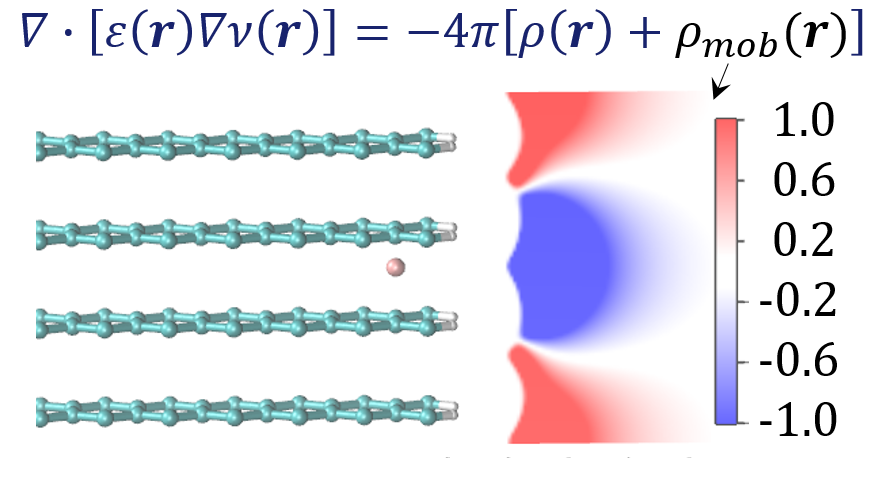
\includegraphics[scale=0.7]{figures/DFT+Continuum.png}
    \caption{DFT simulation of a Lithiated graphite interface in contact with an implicit electrolyte solution based on the solution of Poisson-Boltzmann equation. Reproduced from Ref. \citenum{Dziedzic2020}}
    \label{fig:DFT+continuum}
\end{figure}


\subsubsection{Extracting Stefan-Maxwell diffusivities from MD, and Onsager-Casimir decay of fluctuations hypothesis (MZ)}



\subsubsection{Fitting Potentials for Classical Molecular Dynamics (Lucy)}
\label{sec:potential_fitting}
The development of sufficiently accurate interatomic potentials for a specific chemistry is quite challenging. Interatomic potentials are traditionally based on mathematical functions which has been parameterised using experimental and/or ab-initio derived data. \cite{jones_1924, buckingham_classical_1938} There are a limited number of codes available with the explicit purpose or functionality for fitting potentials. Here, we present a brief overview of some of these codes, linking to more detailed descriptions, before discussing a newly developed code from within the Faraday Institution to highlight the complexities and considerations involved in deriving accurate interatomic potentials.

\textbf{GULP}, the general utility lattice program is a widely used code for performing a variety of simulation types on materials using boundary conditions. \cite{gale_gulp_1997} Within this code, there is the functionality to fit interatomic potentials, to either experimental measurements or first-principles data.\cite{gale_empirical_1996} GULP fits potentials using a "sum of squares" method, which is described as:

\begin{equation}
    F = \sum_{N} \omega ( \,f_{calc}-f_{obs} ) \,^2
\end{equation}

Where $f_{calc}$ and $f_{obs}$ are the calculated and observed quantities and $\omega$ is a weighting factor. The quantities can be a combination of any of the properties that can be calculated for the bulk solid or gas phase molecule including atom positions, cell size, angles, energies, dielectric constant, etc. GULP can fit either to the energy surface or do an empirical fit to structural data. The code is capable of simultaneous fitting to multiple structures and can also handle core-shell models (which capture polarisation of atoms). Further details can be found in reference \citenum{GULP}.

\textbf{Atomicrex} was primarily developed to fit interatomic potential models, written in C++ and Python.\cite{Stukowski_2017} Its capabilities, however, expand to allow for the development of models that describe a given scalar or vector property as a function of atomic configuration. Further details can be found in reference \citenum{Stukowski_2017}.

\textbf{dftfit} is a Python based code for fitting potentials to ab-initio data from DFT calculations including VASP, Quantum Espresso, and Siesta. This code leverages LAMMPS as a calculator, enabling a wide range of potentials to be fitted, and also utilises a range of multi- and single- objective optimizers that are capable of evaluating a potential for properties including energy, forces, stress, lattice constants, elastic constants, bulk modulus, and shear modulus. The main limitation of this code is that its capability of fitting empirical potentials is limited to rigid ion, and can not fit a core-shell model. Further details can be found in reference \citenum{dftfit}.

\textbf{potfit} is another code dedicated to fitting empirical potentials for molecular dynamics. \cite{wen_kim-compliant_2017} Potfit uses a force-matching algorithm to generate the potential from ab-initio data. The code supports three potential types: tabulated, analytic, and OpenKIM potentials, with a range of interaction types, including pair potentials, MEAN, and electrostatics. Similar to dftfit, a limitation of this code is no functionality to fit a core-shell model. Further details can be found in reference \citenum{potfit}.

The above codes have different levels of flexibility and their own unique features, however, during the process of developing potentials for Li(Ni$_x$Mn$_y$Co$_z$)O$_2$ (NMC), and its ternary system LiNiO$_2$, we found that none of these codes are able to accurately develop potentials for these materials. The complex nature of Ni chemistry in a layered-oxide material is challenging, and to the best of our knowledge, no interatomic potentials exist for Ni$^{3+}$, evidenced by a lack of classical MD investigations being published for LiNiO$_2$. In fact, there have only been a limited number of investigations into the LiCoO$_2$ ternary system,\cite{He2019,Hart1998,Fisher2010, Lewis_1985} with a larger number of studies on LiMnO$_2$.\cite{Ledwaba2020, Sayle2005,Ammundsen1999,Dawson0214, Kerisit2014} These articles however are not focused towards the layered-oxide structure. Oxide systems are widely described using a Buckingham form potential, and for the NMC and ternary systems cited here, the Buckingham potentials are presented with varying attributes. Some use rigid ion models, others with core-shell models (introducing polarizability), and a mixture of formal and partial charges have been implemented. With literature in disagreement over which variation of the Buckingham potential is the most accurate for representing the system, our aim was to develop a code capable of fitting different permutations of the Buckingham potential in a modular form.

Structure and composition of a material are crucial to determining the aspects of the potential. For example, a layered structure containing 'sheets' of oxygen, such as LiNiO$_2$, must consider the polarizability. As oxygen is highly polarizable it is desirable to include this in the potential to improved the accuracy of the physics in the system, which is even more important in layered structures where the boundary between interacting atoms is crucial to supporting the structure. In this example, a core-shell model is needed for oxygen, therefore our code needs to allow for a flexible inclusion or exclusion of core-shell interactions for individual atom types within the system. There are predominately two types of core-shell models: the relaxed (massless shells) model and the dynamical (adiabatic shells) shell model.

The relaxed shell model is presented by \citeauthor{Lindan_1993}, \cite{Lindan_1993} where shells have no associated mass and as such their motion is not governed by the usual Newtonian equation, whereas the respective cores are. Because of this, shells respond instantaneously to the motion of the cores, i.e., for any core position, the position of the shell is such that the force is zero. Thus, the energy of the atom is a minimum with respect to the core and shell positions.

The dynamical shell model, more commonly called the adiabatic shell model, was developed by \citeauthor{Mitchell_1993}, \cite{Mitchell_1993} and assigns a fraction of the atomic mass to the shell. There is no defined fraction size, however 10 \% of the atomic mass placed on the shell is common practice. Dynamically, the core-shell atom resembles a diatomic molecule joined by a harmonic bond, however, the high vibrational frequency of the bond prevents effective exchange of kinetic energy between the core-shell atom and the remaining system.

There are benefits and limitations to both these core-shell models, however the adiabatic shell model is less computationally taxing, and therefore beneficial to use for calculating long trajectories, even if considered less accurate. The adiabatic shell model is widely used, including in all the citations relating to the NMC and ternary systems presented in this section. An additional consideration needed when using a core-shell model is the the separation of the formal atomic charge across the core and shell. As there are no consistent trends presented in literature for the charge separation, our code also fits this aspect of the core-shell model.

In some systems, the short-range interactions are overwhelmed by the longer-range coulombic term. In systems such as this, fitting the short-range interactions is equivalent to fitting to noise. In these cases, the system charges can be scaled down to increase the influence of the short-range term, and are termed partial charges. Again, the scaling factor on these charges are system dependent and therefore there is no specific trend, and therefore fitting the charge scaling factor is also useful.

The code we have been developing within the Faraday institution is called \re{BuckFit}, and is currently limited to fitting a Buckingham potential. Although limited to a single potential form, \re{BuckFit} is unique in it's ability to consider all the factors discussed above (rigid ion/core-shell/charge separation/charge scaling) in a modular design, allowing flexible fitting to suit the specific system. The code has been developed in Python and uses a training set consisting of ab-initio data ($Ab$), and utilises the large-scale atomic/molecular massively parallel simulator (LAMMPS). \cite{PLIMPTON19951} The potential is fitted by minimising the mean squared error ($\chi^2$) between the ab-initio forces ($F$) and stress tensors($\sigma$) and those output using the fitted interatomic potential ($IP$), defined as:

\begin{equation}
    \chi^2 = \sum^{N}_{i,\alpha} \frac{(F^{Ab}_{i,\alpha} - F^{IP}_{i,\alpha})^2}{N_i} +  \sum_{\beta} \frac{(\sigma^{Ab}_{\beta} - \sigma^{IP}_{\beta})^2}{6}
\end{equation}

This modular design allows the construction of a Buckingham potential which is able to accommodate the considerations and complexities of different systems. \re{BuckFit} also allows for individual parameters to be fixed/excluded from the fit, lowering the fit dimensionality and computational cost. This is particularly useful for excluding dispersion terms which are known to be zero for a range of elements. Further details of \re{BuckFit} can be found \re{here [cite]}.

\subsection{Calculating observable properties.}
Anything slightly more specific here. We could also have the schematic of the properties at different length scales?

\subsubsection{Equilibrium voltage (Mike)}
\label{sec:properties_equilibriumvoltage}
The equilibrium cell voltage, $E(x)$, is a fundamental thermodynamic quantity related to the energy density of a cell \cite{urban_computational_2016,CEDER1999131,VanderVen2020}. In a lithium ion cell, $0 < x < 1$ denotes the fraction of sites occupied by lithium in the intercalation host. In experimental measurements of lithium ion cells, $E(x)$ can be probed through measurements of the open circuit voltage (OCV), that is, the voltage between the cathode and anode terminals under zero current flow, assuming that the system has been given sufficient time for the OCV to relax to the value of $E(x)$. The equilibrium cell voltage can be modelled through \textit{First Principles} calculations at $T = 0$ K \cite{urban_computational_2016,CEDER1999131,VanderVen2020}; the effect of thermal fluctuations can be included by modelling using Monte Carlo calculations \cite{mercer_influence_2017,Kim2001h}.

There is a fundamental relationship between the Gibbs free energy of lithium dissolution into the host, $G(x)$, the chemical potential of Li intercalation in the host, $\mu(x)$, and the cell voltage $E(x)$. Knowledge of $G(x)$ also provides information about the evolution of the phase behaviour dependent on the fraction of intercalated Li \cite{CEDER1999131,persson2010,VanderVen2020,VanDerVen2000b}, enabling the construction of phase diagrams from\textit{First Principles}. The relationships are represented schematically in Figure~\ref{fig:vanderven_thermodynamics} and are subsequently shown more formally. In essence: the tangent to the free energy curve, $G(x)$ allows the $\mu(x)$ and hence the cell voltage to obtained. Alternatively, integration of $\mu(x)$ can be used to derive free energy curves. 

\begin{figure}
    \centering
    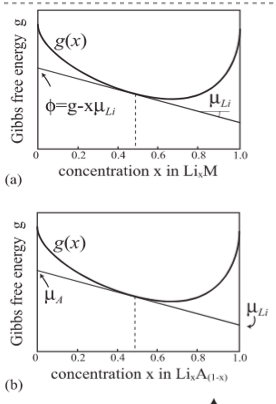
\includegraphics[scale=2]{figures/thermodynamics_vanderven.png}
    \caption{Representation of the connection between the Gibbs free energy, $G(x)$, the  lithium chemical potential $\mu(x)$ in (a) an intercalation electrode and (b) an alloy electrode. Reproduced from \cite{VanderVen2020}}
    \label{fig:vanderven_thermodynamics}
\end{figure}

In the case of a lithium ion cell the equilibrium cell voltage, $\phi(x)$ and chemical potential of intercalated Li, $\mu(x)$ are related as

\begin{equation}
    \phi(x) = -\frac{\mu(x) - \mu_{\rm{Li}}^{\rm{ref}}}{nF},
    \label{eq:potchempot_raw}
\end{equation}
where $\mu_{\rm{Li}}^{\rm{ref}}$ is the chemical potential of the reference electrode, $n$ is the number of electrons transferred per formula unit of intercalation host ($n =1$ for Li-ion cells), and $F$ is the Faraday constant. The most convenient reference potential, both from the point of view of simulations and also to compare with experimental measurements of Li-ion half cells, is the bcc metallic Li anode.  With a suitable choice of units for all potentials ($\mu$ expressed in eV per formula unit of intercalation host), equation~\ref{eq:potchempot_raw} can be written much more simply as \cite{CEDER1999131}
\begin{equation}
    \phi(x) = -\mu(x).
    \label{eq:potchempot}
\end{equation}

The intercalated Li chemical potential is defined by

\begin{equation}
    \mu(x) = \left(\frac{\partial{\underline{G}(x)}}{\partial{N_{Li}}}\right)_{p,T,N_{\rm{host}}} = \left(\frac{\partial{G(x)}}{\partial{x}}\right)_{p,T,N_{\rm{host}}},
    \label{eq:chemicalpotgibbs}
\end{equation}
where $\underline{G} =$ the absolute (i.e. extensive) Gibbs free energy of Li dissolution into the host, $p =$ pressure, $T =$ the absolute temperature, $N_{\rm{host}}$ and $N_{\rm{Li}}$ are respectively the number of host and lithium atoms in the system. The subscripts $p$, $T$ and $N_{\rm{host}}$ will be implicitly assumed constant from now on and dropped to simplify notation.

Likewise it is well known that
\begin{equation}
    \frac{\partial{G(x)}}{\partial{x}} = \frac{\partial{H(x)}}{\partial{x}} - T\frac{\partial{S(x)}}{\partial{x}}, 
    \label{eq:gibbshs}
\end{equation}
where $H(x)$ and $S(x)$ are the enthalpy and entropy, respectively, per formula unit of host material.

We can use equations \ref{eq:potchempot}, \ref{eq:chemicalpotgibbs} and \ref{eq:gibbshs} to get $\partial{G}/\partial{x} = -E_{\rm{OCV}}$. Then, taking the derivative of the OCV with respect to $T$ and using the chain rule, we obtain 

\begin{equation}
   \frac{\partial{E_{OCV}(x)}}{\partial{T}}
  = \frac{\partial{S(x)}}{\partial{x}} - \frac{\partial}{\partial{x}}\left[{T}\left(\frac{\partial{S(x)}}{\partial{T}}\right)_{p,N_{host}}-\left(\frac{\partial{H(x)}}{\partial{T}}\right)_{p,N_{host}}\right].  
   \label{eq:entropy_measurement_extra}
\end{equation}

It then follows that

\begin{equation}
   \frac{\partial{S(x)}}{\partial{x}} = \frac{\partial{E_{\rm{OCV}}(x)}}{\partial{T}}
    \label{eq:entropy_measurement}
\end{equation}
and so
\begin{equation}
    \frac{\partial{H(x)}}{\partial{x}} = T\frac{\partial{E_{\rm{OCV}}(x)}}{\partial{T}} - E_{\rm{OCV}}(x).
    \label{eq:enthalpy_measurement}
\end{equation}

Due to the choice of units of eV per formula unit for the potentials $H(x)$ and $TS(x)$, i.e. as in the conversion between equations~\ref{eq:potchempot_raw} and \ref{eq:potchempot}, the usual factors of $F$ have been omitted. In this way it is possible to simulate not only the equilibrium voltage, but split its contributions into enthalpy and entropy components. Both components can be experimentally measured \cite{schlueter_quantifying_2018,Mercer2019,THOMAS2003844,Reynier2004,Yazami_2006} and modelled through Monte Carlo or mean field methods \cite{schlueter_quantifying_2018,mercer_influence_2017,Mercer2019,GavilanArriazu2017}, providing additional properties for model validation purposes and to check the temperature dependence of those properties is modelled accurately. A good thermodynamic basis can then be used to derive dynamic properties as outlined in the subsequent sections.

\subsubsection{Thermodynamic Enhancement Factor (Arihant)}
\label{sec:tf}
The thermodynamic enhancement factor $\chi$ describes the transport in electrolytes and how the variation in concentration in an electrolyte leads to a drop in open-circuit voltage across it.\cite{Stewart2008, wang2020} The thermodynamic factor is related to the activity coefficient $\gamma_{\rm mean}$ of electrolyte as:

\begin{equation}
    \label{eq:tf}
    \chi = 1+\frac{\delta \ln \gamma_{\rm mean}}{\delta \ln \cif}
\end{equation}

The activity coefficient of electrolytes can be computed from DFT+\pbe{} models described in section \ref{sec:dft+cont}.\cite{Ringe2016, Dziedzic2020} The activity coefficient describes behavior of non-ideal electrolytes, and the dependence of their chemical potentials on electrolyte concentration.\cite{Atkins2014}

\begin{equation}
    \label{eq:mujid}
    \mu_j\left[\{\cif\}\right]=\mu_j\left[\{\cif=0\}\right]+ \kb T\ln{\gamma_j},  \ j=1\dots p
\end{equation}

%where $x_j$ is the mole fraction of the quantum solute $j$. For a non-ideal electrolyte solution, the non-ideality can be incorporated by using the activity $a_j=x_j\gamma_j$, 
%where $\gamma_j$ is the activity coefficient of the solute $j$ at electrolyte concentration $\{\cif\}$.
%\begin{equation}
%\label{eq:mujnid}
%\mu_j^{\textrm{non-id}}\left[\{\cif\}\right]=\mu_j\left[\{\cif=0\}\right]+ R T\ln{x_j\gamma_j},
%\end{equation}
The chemical potential of the quantum solute represents the change in the free energy per number of molecules ($n_j$) of solute:

\begin{equation}
    \label{eq:dtdn}
    \frac{\partial \Omega}{\partial n_j}\bigg|_{\{\cif\}}=\frac{\partial \Omega}{\partial n_j}\bigg|_{\{\cif=0\}}+ \kb T\ln{\gamma_j}, \ j=1\dots p
\end{equation}

%for a single atom of solute in a cell, ($x_j=1$):
%\begin{equation}
%\label{eq:sdtdn}
%\Omega\left[\dens\ofrvec, {\{\cif\}}\right] -\Omega\left[\dens\ofrvec=0, {\{\cif\}}\right] = \Omega\left[\dens\ofrvec, {\{\cif=0\}}\right] -\Omega\left[\dens\ofrvec=0, {\{\cif=0\}}\right]+ \kb T \ln{\gamma_j},
%\end{equation}
which can be written in terms of solvation energies because the energies of solute $j$ in vacuum cancel out:

\begin{equation}
    \label{eq:dtc}
    \Delta\Omega_j\left[{\{\cif\}}\right]-\Delta\Omega_j\left[{\{\cif=0\}}\right]=\kb T \ln{\gamma_j}, \ j=1\dots p
\end{equation}

or, equivalently

\begin{equation}
    \label{eq:activityj}
    \frac{\Delta\Delta\Omega_j\left[\{\cif\}\right]}{\kb T} =\ln{\gamma_j}, \ j=1\dots p.
\end{equation}

Hence, activity coefficients can be computed from the electrolyte effect on solvation energies ($\Delta\Delta\Omega$), which is described in section \ref{sec:dft+cont}. The mean activity coefficient of all the $p$ electrolytes species can be calculated as:
\begin{equation}
    \label{eq:activitymean}
    \ln \gamma_{\rm mean} = \frac{1}{p}\sum_{j=1}^p \ln \gamma_j.
\end{equation}

\subsubsection{Diffusion coefficients (Lucy/Maxim)}
\begin{itemize}
    \item What is meant by diffusion coefficient. This term means different things to atomistic and contiuum modellers. In Van der Ven's review, they briefly mention the different ways of calculating the different diffusion coefficients so it might be nice to briefly mention them here as well, and also refer to their review.
    \item microscopic diffusion and macroscopic diffusion as sections.
    \item Go through each "type" of diffusion coefficient and discuss how to calculate and what methods to use. Possibly the pros/cons of each and even how this relates to continuum model scale. (Maxim mentions this is important)

    \re{Rana add paper and book reference here if you can}
\end{itemize}

\subsubsection{Thermal, electronic, and vibrational properties}
Lead: Hui
\begin{itemize}
    \item Electronic behaviour links to the work and methods which Chris Savoury (David Scalon's group, UCL) are working on.
    \item vibrational properties, chemical trends in vibrational properties 
    \item thermal properties/ heat management
\end{itemize}

Traditional crystallography often leads to the image of atoms being held in static positions through stiff chemical bonds, while atoms must be vibrating within crystals and it is the natural interpretation of temperature. Thus we need to understand lattice dynamics in order to have a complete picture of crystalline materials. Lattice dynamics of a crystal has been widely used in vibrational spectra and thermal transport.

The lattice thermal conductivity of a crystalline material ($\kappa$) 
depends on the nature of its heat-carrying vibrations.
Formally, each phonon mode makes a contribution to the macroscopic thermal conductivity given by the product of the modal heat capacity ($C_V$), the group velocity ($v$), and the phonon mean free path ($v \times \tau$, where $\tau$ is the phonon lifetime).
The macroscopic $\kappa$ is obtained by summing over band indices ($v$), averaging over wavevectors ($q$) and normalizing by the cell volume:
%
\begin{equation}
 \kappa = \frac{1}{NV_0} \,\sum_{qv} C_{V,qv} v_{qv} \otimes v_{qv} \tau_{qv} \label{eqn1}
\end{equation}
%
where $N$ is the number of unit cells in the crystal (equivalent to the number of wavevectors included in the Brillouin zone summation) and $V_0$ is the volume of the crystallographic unit cell.

The heat capacity and group velocity can be determined from the harmonic phonon dispersion while the lifetime of each phonon mode could be computed within phonon many-body perturbation theory by taking into account the leading term of three-phonon scattering processes.\cite{togo_distributions_2015}


%However,

%\begin{equation}
%    {T}\left(\frac{\partial{S(x)}}{\partial{T}}\right)_{p,N_{host}} = %\left(\frac{\partial{H(x)}}{\partial{T}}\right)_{p,N_{host}} = C_{p},  
%    \label{eq:heat_capacity}
%\end{equation}
%where $C_{p}$ is the specific heat capacity at constant pressure. Hence we can %simplify equation~\ref{eq:entropy_measurement_extra} as


% \subsubsection{Electric conductivity}

\section{Anodes (Mike/Chao/Arihant/Rana/Denis?)}
\subsection{Introduction and historical context}
- lead: (Mike: I am happy to take the lead on this part (dependent on scope) in exchange for others helping on the anode bulk part)
- review: Chris/all
N.B. there is a recently published historical overview on anodes that we can mostly paraphrase and condense in this part in ref. \citenum{asenbauer_success_2020}.

Historical overview: RSC magazine historical overview

\subsection{Bulk Properties}
\label{sec:anode_bulk}

\subsubsection{Equilibrium potential, open circuit voltage (OCV) and graphite staging}
\label{sec:anodes_ocv}
- lead: Mike
- review: Chao/Denis

Mike: I propose to include a diagram of experimental OCV first together with schemes of the staging from my own papers \cite{Mercer2019}.

    \begin{figure}
    \centering
    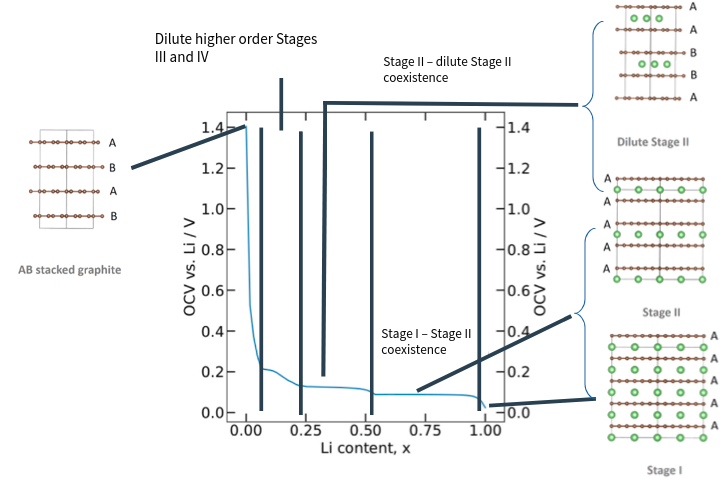
\includegraphics[scale=2.3]{figures/exptocv_staging.png}
    \caption{Illustration of OCV features of lithium in graphite using from ref. \citenum{Mercer2019}. Flat regions are linked to two phase coexistence of reported stages. Reproduced from Ref. *}
    \label{fig:expt_ocv}
\end{figure}

We can also add Kristin Persson's work - still the most comprehensive phase diagram of lithium in graphite and includes 0K OCV \citenum{persson2010}, although I have some criticisms of it. 

    \begin{figure}
    \centering
    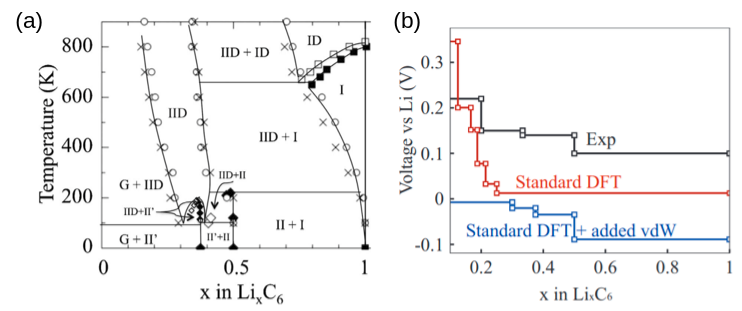
\includegraphics[scale=2]{figures/perrson_phasediagram.png}
    \caption{(a) Phase diagram of lithium in graphite, determined by performing Monte Carlo calculations parameterised by effective cluster interactions from DFT calculations. (b) zero kelvin equilibrium potential profiles dependent on different levels of van der Waals corrections. From ref. \citenum{persson2010}}
    \label{fig:persson_graphitephases}
\end{figure}

\begin{itemize}
    \item The voltage profile and "stage" formation
    -ref. \citenum{persson2010},\citenum{VanderVen2020}
    \item Phase diagram:  open circuit voltage (DFT $\rightarrow$ cluster expansion $\rightarrow$ MC, from Kristin Persson's paper). Phase diagram ref. \citenum{persson2010}
    \item DFT only gives 0 K behaviour - need for input at longer length scales from MC, kMC to put in entropy and model dynamic behaviour
\end{itemize}

\subsubsection{Ion diffusion in Li-GICs} 
\label{sec:anodes_ion_diffusion}
- lead: Rana

suggested action MM: Mike and Rana write these sections independently at first (but we will have discussed what we want to write). Once complete, we merge into a single section.
Due to high lithium intercalation capacity (372 mAh/g), lithium−graphite intercalation compounds (Li-GICs) are used as active negative electrodes in commercial Li-ion batteries. Graphite intercalation compounds are classified by a stage index n denoting the number of graphite layers between adjacent intercalate layers. A stage index n → ∞, therefore, refers to pure graphite. In the present part, we are focusing on three structures of LiC$_{6n}$ (n = 1, 2) namely LiC$_6$, stacking st-LiC$_6$, and LiC$_{12}$ ref. \citenum{RanaLiC6}. 

We have calculated the structural, energetic, electronic properties, defect properties, and cation diffusion mechanisms in the Li-GICs employing dispersion-corrected DFT method. According to our investigation ref. \citenum{RanaLiC6}, the interlayer interactions due to the van der Waals forces play an effective role in graphite and LiC$_{6n}$ compounds. 

\begin{figure}
    \centering           
    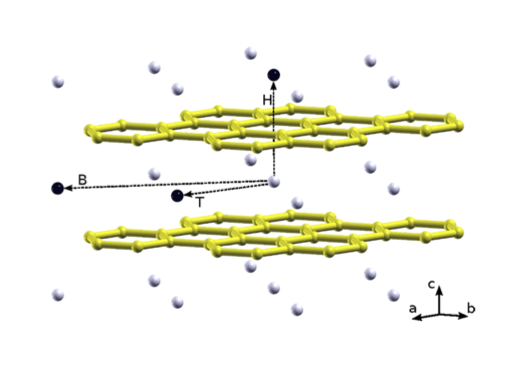
\includegraphics[scale=0.8]{figures/Islam-Fig-LiC6.png}
    \caption{Li migration pathway in LiC$_{6}$. In the through-plane pathway, lithium migrates through a carbon hexagon hollow (H) along the crystallographic c direction. The in-plane pathways are denoted as bridge (B) and top (T) ref. \citenum{RanaLiC6}}
    \label{fig:Rl}
\end{figure}
        
We have performed various kinds of ion diffusion mechanisms.i.e, Li ion diffusion through a carbon hexagonal hollow (H) pathway which is denoted as the migration along c direction and in plane migrations as denoted as bridge (B) and top (T) migration pathways ref. \citenum{RanaLiC6}. Our study shows that Li diffusion along the crystallographic c direction is prohibited due to a large activation energy barrier. Whereas, Li diffuses in the ab plane with a small energy barrier.

\subsubsection{kMC approaches to Li-graphite}
\label{sec:anodes_kmc}
-lead: Mike

- lead: Mike + Rana
- review: Chao/Denis

\begin{itemize}
    \item Persson et al. ref. \citenum{persson2010}
    \item + Rana's LixC6 paper ref. \citenum{RanaLiC6} Merge later
    \item recent kinetic Monte Carlo (kMC) work by Leiva group, e.g. ref. \citenum{gavilan-arriazu_kinetic_2020}, ref. \citenum{gavilan-arriazu_effect_2020}, including temperature effects, exchange current density, dynamic electrochemistry.
\end{itemize}

    \begin{figure}
    \centering
    \includegraphics[scale=2]{figures/kmc_scheme.png}
    \caption{Representation of insertion and diffusion of lithium in graphite in kMC model.  From \citenum{gavilan-arriazu_effect_2020}}
    \label{fig:graphite_kmcscheme}
\end{figure}

    \begin{figure}
    \centering
    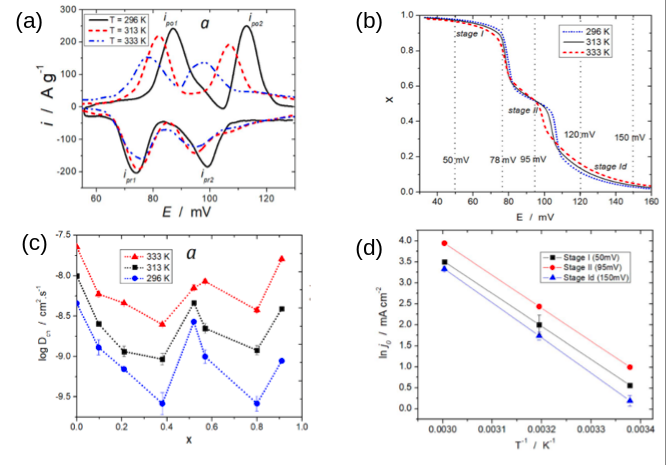
\includegraphics[scale=2]{figures/kmc_observables.png}
    \caption{Effect of temperature on dynamic behaviour of lithium insertion in graphite. (a) voltammograms (b) voltage profiles (isotherms) (c) diffusion coefficients, (d) exchange current density. insertion and diffusion of lithium in graphite in kMC model.  From \citenum{gavilan-arriazu_effect_2020}}
    \label{fig:graphite_kmcobservables}
\end{figure}

\subsubsection{Entropy}
\label{sec:anodes_entropy}
-lead: Mike
I could alternatively write a section on this topic in cathodes on LMO \citenum{mercer_influence_2017,schlueter_quantifying_2018}.
Could add some figures from mean field paper \citenum{Mercer2019} as an example of modelling the configurational entropy by two level approach
- lead: Mike
-review: Hui (phonons)

    \begin{figure}
    \centering
    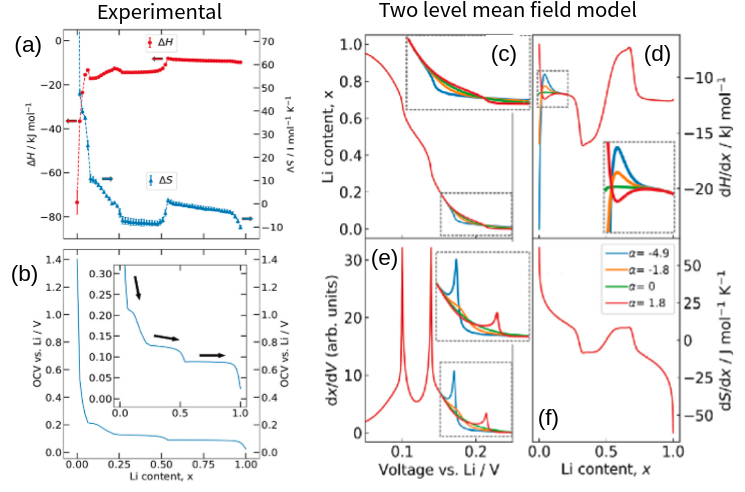
\includegraphics[scale=2]{figures/graphite_meanfield_alpha.png}
    \caption{(a) experimental partial molar enthalpy and entropy profiles obtained during galvanostatic discharge of Li/graphite coin cells. (b) Experimental OCV. Mean field simulations of thermodynamic profiles: (c) Simulated OCV, (d) partial molar enthalpy, (e) dQ/dV (or voltammogram) (f) partial molar entropy. Results are shown dependent on different correction amplitudes, $\alpha$.  Reproduced from Ref. \citenum{Mercer2019}}
    \label{fig:graphite_meanfield}
\end{figure}
\begin{itemize}
    \item configuration entropy
    \item electronic behaviour, link to dilute Li transitions ref. \citenum{Mercer2019}. Lack of implications for measureable entropy.
\end{itemize}

%\subsubsection{Hysteresis}  % To be mentioned as a challenge in outlook.
%- lead: Mike
%- review: Chao/Denis

%N.B. Mike: this paper is still in review in Nat. Comm.. I will have a better idea soon, once reviewer reports are back, whether it is likely this will be published in time for December. In any case, I will write this section last. If not, we can mention aspects of hysteresis in outlook.
%\begin{itemize}
%    \item hysteresis (in review, Nat. Comm.): including shifts in carbon layers. Draw links with similar calculations done on cathode ref. \citenum{radin_role_2017}
%    \item barriers to transition between different stages.
%\end{itemize}

%\subsubsection{Outlook}



\subsection{Surfaces and Interfaces (Arihant/Chao/Rana)}
\label{sec:anodes_surfaces_interfaces}
% Chao: Here are some suggestions to this section

\subsubsection{Possible graphite surfaces and their stability}
- lead: Rana + separate outlook to be merged later

- Rana's paper: {basal plane(001), very high barrier}; {Non-basal plane, (100), (010), or the armchair, zigzag edge, much lower barrier}
    
- Stability: basal on the surface energies for different surfaces, Wuff Shape, etc.

\subsubsection{the surface effect on Li intercalation}
- lead: Chao + separate outlook to be merged later

\begin{itemize}
    \item \textbf{surface effect on intercalation energy} 

    \iffalse
    Focus on the non-basal plane(e.g. armchair edge and zigzag edge) and introduce their effects on Li intercalation energies at dilute limit. (If the concentration paper is ready in time, we can also add more discussion here.)
    \fi
    
    Understanding the nature of Li diffusion in graphite is of importance to optimize material designs. As described above, the bulk diffusion properties of Li has been widely investigated.\cite{persson2010,toyoura2008first,toyoura2010effects,yao2012diffusion,thinius2014theoretical} However, the edge morphology, which might also highly affect the intercalation of Li, has been rarely discussed due to the complicated structures of the interface between the graphite and the electrolyte.
    Uthaisar et al. studied the Li adsorption and diffusion on the edged graphene system from the DFT perspective.\cite{uthaisar2010edge} The graphene edges were found not only affecting Li adsorption but also the diffusion coefficient. The narrower graphite nanoribbons shows faster discharge behaviour than the larger sized graphene due to edge effects.
    Furthermore, experiments reported Li chemical diffusivities in graphite ranging from 10$^{-6}$\sim10$^{-14}$ cm$^2$/s.\cite{toyoura2010effects} Whereas, the DFT calculations based on bulk graphite indicates that Li diffusion coefficents at stage-II and stage-I are around 10$^{-7}$ cm$^2$/s and decrease very slightly with Li concentration increasing.\cite{persson2010}  The wide range of experimentally measured diffusion coefficients could be referred to the high anisotropy of the layered material and sizes of graphite particles.
    Therefore, in-depth understanding of interface effects would allow to tune the interface properties so that to improve the charging/discharging rates and rationally optimize the battery performance.

    \begin{figure}
        \centering
        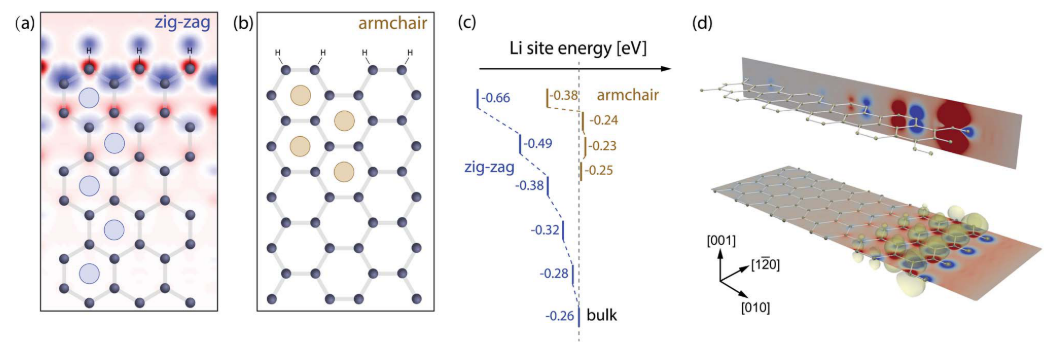
\includegraphics[scale=0.5]{figures/Intercalation energies.PNG}
        \caption{Geometrical structures of graphite edges for zigzag-edged graphite (a) and armchair-edged graphite (b). (c) is the profile of Li adsorption energies as a function of distance from the edge towards the bulk of graphite. (d) Illustrates the spin densities in zigzag-edged graphite. The iso-surface value is 0.0002 e/${\AA}^3$. Reproduced from Ref.~\citenum{peng2020lithium}.}
        \label{fig:arm_zig}
    \end{figure}
    
    Recently, different edged graphites at dilute Li concentration were comprehensively investigated using DFT calculations.\citenum{peng2020lithium} Interestingly, the unique electronic structure near the edges was identified, particularly near the zigzag edge, induces the different intercalation energies of Li in graphite. Figure~\ref{fig:arm_zig} shows the Li intercalation at the armchair-edged and zigzag-edged graphite, respectively. The adsorption energy is expressed as follows: $E_{ads}$= E(Li$|$Graphite)-E(Graphite)-E(Li), where E(Li$|$Graphite), E(Graphite), E(Li) are the energies of lithiated graphite, the pristine graphite and one Li in BCC Li metal, respectively. At the armchair edge, from the energy profile (cf. Figure~\ref{fig:arm_zig}), the adsorption energy of Li is the lowest at the edge site (-0.38 eV). With Li penetrating into the bulk, the adsorption energy decreases rapidly to -0.24 eV at the sub-surface site and becomes -0.26 eV at the bulk site. The topological geometry of armchair edge promotes Li adsorption relative to the graphite bulk.
    At the zigzag edge, the edge effect even becomes much stronger as the identified surface state on the edged carbons.
    Figure \ref{fig:arm_zig} shows that Li achieves a much lower adsorption energy of -0.66 eV at the zigzag-edge site, indicating the strong binding of Li at the edge site. The edge effect in the zigzag system is much stronger than that at the armchair edge. In the zigzag system, the edge effect also penetrates into the bulk, indicated by the gradually decreasing Li adsorption energies in magnitude from the edge to the bulk. 
    
    The electronic structure analysis in their work shows that The zigzag edge displays a completely different spin densities contributed by the $p_z$ orbitals perpendicular to the graphene plane (see Figure \ref{fig:arm_zig} a and d). These spin densities consist of the unpaired electrons accumulating on the edged carbons. The amplitude of this topological surface state gradually diminishes over a few bond distances beneath the surface. It is this surface state that interacts with Li at the zigzag edge and favors its adsorption. In summary, the adsorption energies near the zigzag edge are much larger than in the bulk or near the armchair edge due to the surface state which favors Li adsorption by accepting electrons from Li to the graphene host.

    
    \item \textbf{the surface effect on Li incalation kinetics}

    Discuss different edge effects on Li diffusion including the diffusion barrier and diffusion rate
    
    \begin{figure}
        \centering
        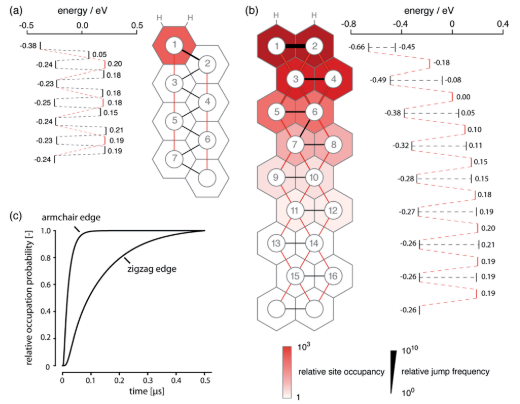
\includegraphics[scale=0.5]{figures/Graphite_edge_effects.PNG}
        \caption{Li diffusion at (a) armchair-edged and (b) zigzag-edged graphite. Colored hexagons indicate site occupancy relative to bulk and the width of the lines connecting sites indicates jump frequency; (c) probability for Li to occupy a site approximately 20 \AA below the surface relative to the steady-state value after being introduced at time zero at the edge.Reproduced from Ref.\citenum{peng2020lithium}}
        \label{fig:my_label}
    \end{figure}
    
    \item \textbf{Modification of graphite material to enhance the charging rate}
\end{itemize}

\subsubsection{the solid-liquid interface: (Li desolvation/solvation at graphite/electrolyte interface}
- lead: Arihant + separate outlook to be merged later

\begin{itemize}
    \item the free energy change using the implicit solvent model Ref.\citenum{haruyama2018}
    
    \begin{figure}
        \centering
        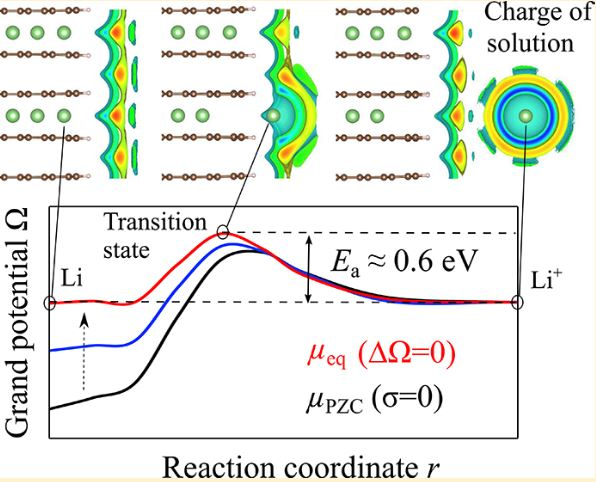
\includegraphics[scale=0.75]{figures/graphite-interface.JPG}
        \caption{Li-ion transfer at the graphite-implicit solution interface, Ref. \citenum{haruyama2018} }
        label{fig:my_label}
    \end{figure}
    
    \item the free energy change using the classical MD  simulation Ref.\citenum{ohwaki2018}
    \item Comparison between different methods and discussion for advanced solvent model development
    \item new developed method (from Chris' group?)
    \item \textbf{Addressing the limiting step for graphite anode charging/discharging and outlook for material design}
\end{itemize}

\subsubsection{Graphite Surfaces}
Graphite is widely used as anodes (in the form of Li-GICs) in Li ion batteries. In literature, most of the theoretical and experimental papers are devoted for (001) surface investigation. Since it is well known that Li diffusion through the (001) planes is hindered by large barriers \cite{RanaLiC6}, Li intercalation of graphite particles must proceed either via defects in the (001) plane or via the open non-(001) surfaces. This prompted us to revisit the surface properties on various low index graphite surface planes namely (001), (110), (101), (111) and (100) \cite{Rana-Graphite-Surf}. The calculations were performed using pure DFT and dispersion corrected DFT approaches. According to this investigation, we have observed the following things:
\begin{itemize}
    \item According to the calculated surface energy, the stabilization of non-reconstructed graphite surface planes ranges as (001) $>$ (110) $>$ (111) $>$ (101) $>$ (100).
    \item Two different types of surface reconstruction configurations are observed, such as, oval (o) and sinusoidal (s).
    \item The reconstructed surfaces are more stable that the unreconstructed surfaces 
    \item According to the Gibbs–Wulff theorem, 88.3 \% , 6.3 \%, 4.5 \% and 0.8 \% of the crystal surface area represents for the (001), (101), (110) and (111) surfaces, respectively.  
    \item The (001) surface dominates over all other surfaces whereas the (100) surface does not contribute significantly to the overall crystal surface
\end{itemize}
\begin{itemize}
    \item solid side properties (anode surface)
    \begin{itemize}
        \item Surface analysis of graphite ref. \citenum{Rana-Graphite-Surf}
        \item intercalation energy

        \item diffusion properties

        \item Chao's edge effects paper
        \item influence of functional groups
        
        \begin{figure}
            \centering            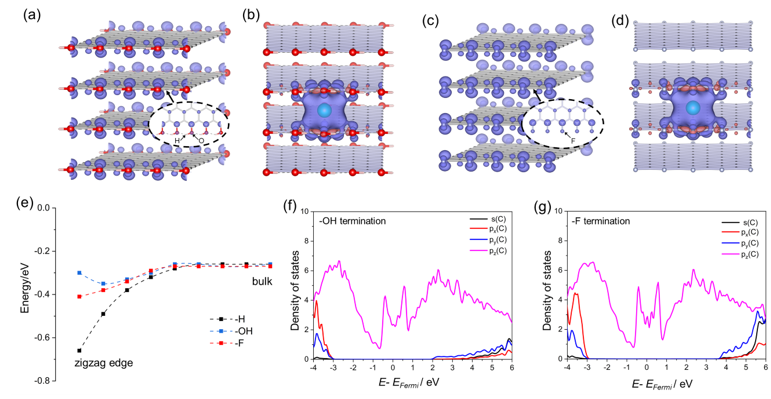
\includegraphics[scale=0.5]{figures/functional groups.PNG}
            \caption{(a) shows the spin density accumulation on the edged carbon in OH-terminated zigzag-edged graphite. The inserted graph shows the top view of the basal plane of graphite edge. The iso-surface value is 0.003 eV/Å3. (b) is the charge density difference of Li adsorption at the edged site in zigzag-edged graphite. (c) is the spin density in F-terminated zigzag-edged graphite. The inserted graph shows the top view of the basal plane of graphite edge. The iso-surface value is 0.0015 eV/Å3. (d) is the charge density difference of Li adsorption at the edged site in F-terminated graphite. The iso-surface value is 0.001 eV/Å3. (e) shows Li adsorption energy change from the edged site to the bulk site in zigzag-edged graphite with different terminations on edged carbons. (f) and (g) are the local density of states (LDOSs) of edged carbons in OH-terminated and F-terminated zigzag-edged graphite.Reproduced from Ref.xx}
            \label{fig:my_label}
        \end{figure}
    \end{itemize}
    \item Solvent/electrolyte effect 
    \begin{itemize}
        \item the solvation/desolvation kinetics of ion at the interface.Ref. \citenum{haruyama2018,ohwaki2018}
        
        \begin{figure}
            \centering
            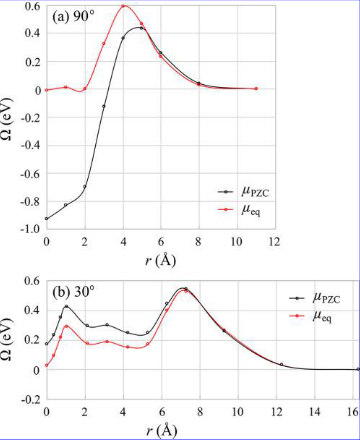
\includegraphics[scale=0.5]{figures/desolvation_implicitmodel.PNG}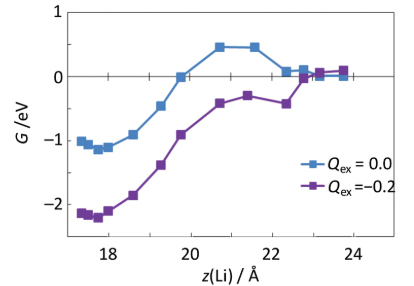
\includegraphics[scale=0.5]{figures/desolvation_MD.PNG}
            \caption{Caption}
            \label{fig:my_label}
        \end{figure}
        
        \item Discuss interface papers: (DFT+implicit electrolyte solution): Ref. \citenum{haruyama2018, Dziedzic2020}
    \end{itemize}
\end{itemize}

\subsection{Outlook and challenges for anodes}
- all: but each to overview their own sections

Make this a general outlook and challenges of anodes?
\begin{itemize}
    \item Better quality functionals to describe van der Waals interactions, 
    \item explicit determination of energetic barriers to shifting carbon layers, 
    \item role of configurational entropy in hysteresis 
    \item modelling higher order graphite stages
    \item surface and interface effects: c.f. the next section
    \item anode materials other than graphite, such as silicides
\end{itemize}

\section{Electrolytes (Maxim/Arihant/Rana/Chris/Lucy)}
\subsection{Introduction and historical context}
General picture and types of electrolytes. The importance of moving from liquid to solids and the challenges involved.
General description, broad picture

\subsection{Liquid Electrolytes (Maxim and Arihant)}
\subsubsection{Introduction/Background}
Literature review with examples of different liquid electrolytes
\begin{itemize}
    \item ionic conductivity and 
    \item diffusion coefficients
    \item Green-Kubo
    \item Stefan-Maxwell approach
    \item general solvation structures in electrolytes
\end{itemize}

\subsubsection{Activity coefficients of electrolytes}
The charge transport in electrolytes is described by their activity coefficients which can be calculated from DFT simulations of solutes in electrolyte solutions as described sec.\ref{sec:tf} A sample calculation of activity coefficient of LiPF$_6$ in ethylene carbonate solvent is discussed here from Ref. \citenum{Dziedzic2020}. The experimental values of bulk permittivity of ethylene carbonate (EC) ($\eps^\infty=90.7$)\cite{Hall2015} and surface tension of EC (0.0506~N/m),\cite{Naejus2002} are taken from the literature. The solvent radius is set to $R^\textrm{solvent}_k= 10.5~a_0$ to approximate the size of an EC molecule, and the isovalue of solute electronic density ($\denselec^\acc$) is varied to match the experimental activity coefficients. The plot of the computed activity coefficients as a function of the square root of electrolyte concentration in Figure~\ref{fig:ac} along with experimental values from literature.\cite{Stewart2008} We see a good match for $\denselec^\acc=0.002~e/a_0^3$. Trends are also plotted from the linearized approximation of P-BE where the solvent radius is reduced to show the behavior of point charges from the Debye-H\"uckel theory.\cite{debye1923theory} The thermodynamic factor can be obtained from numerically differentiating these curves by using eq. \eqref{eq:tf}. This is a novel technique of calculating activity coefficients and thermodynamic factors from atomistic methods.

\begin{figure}
    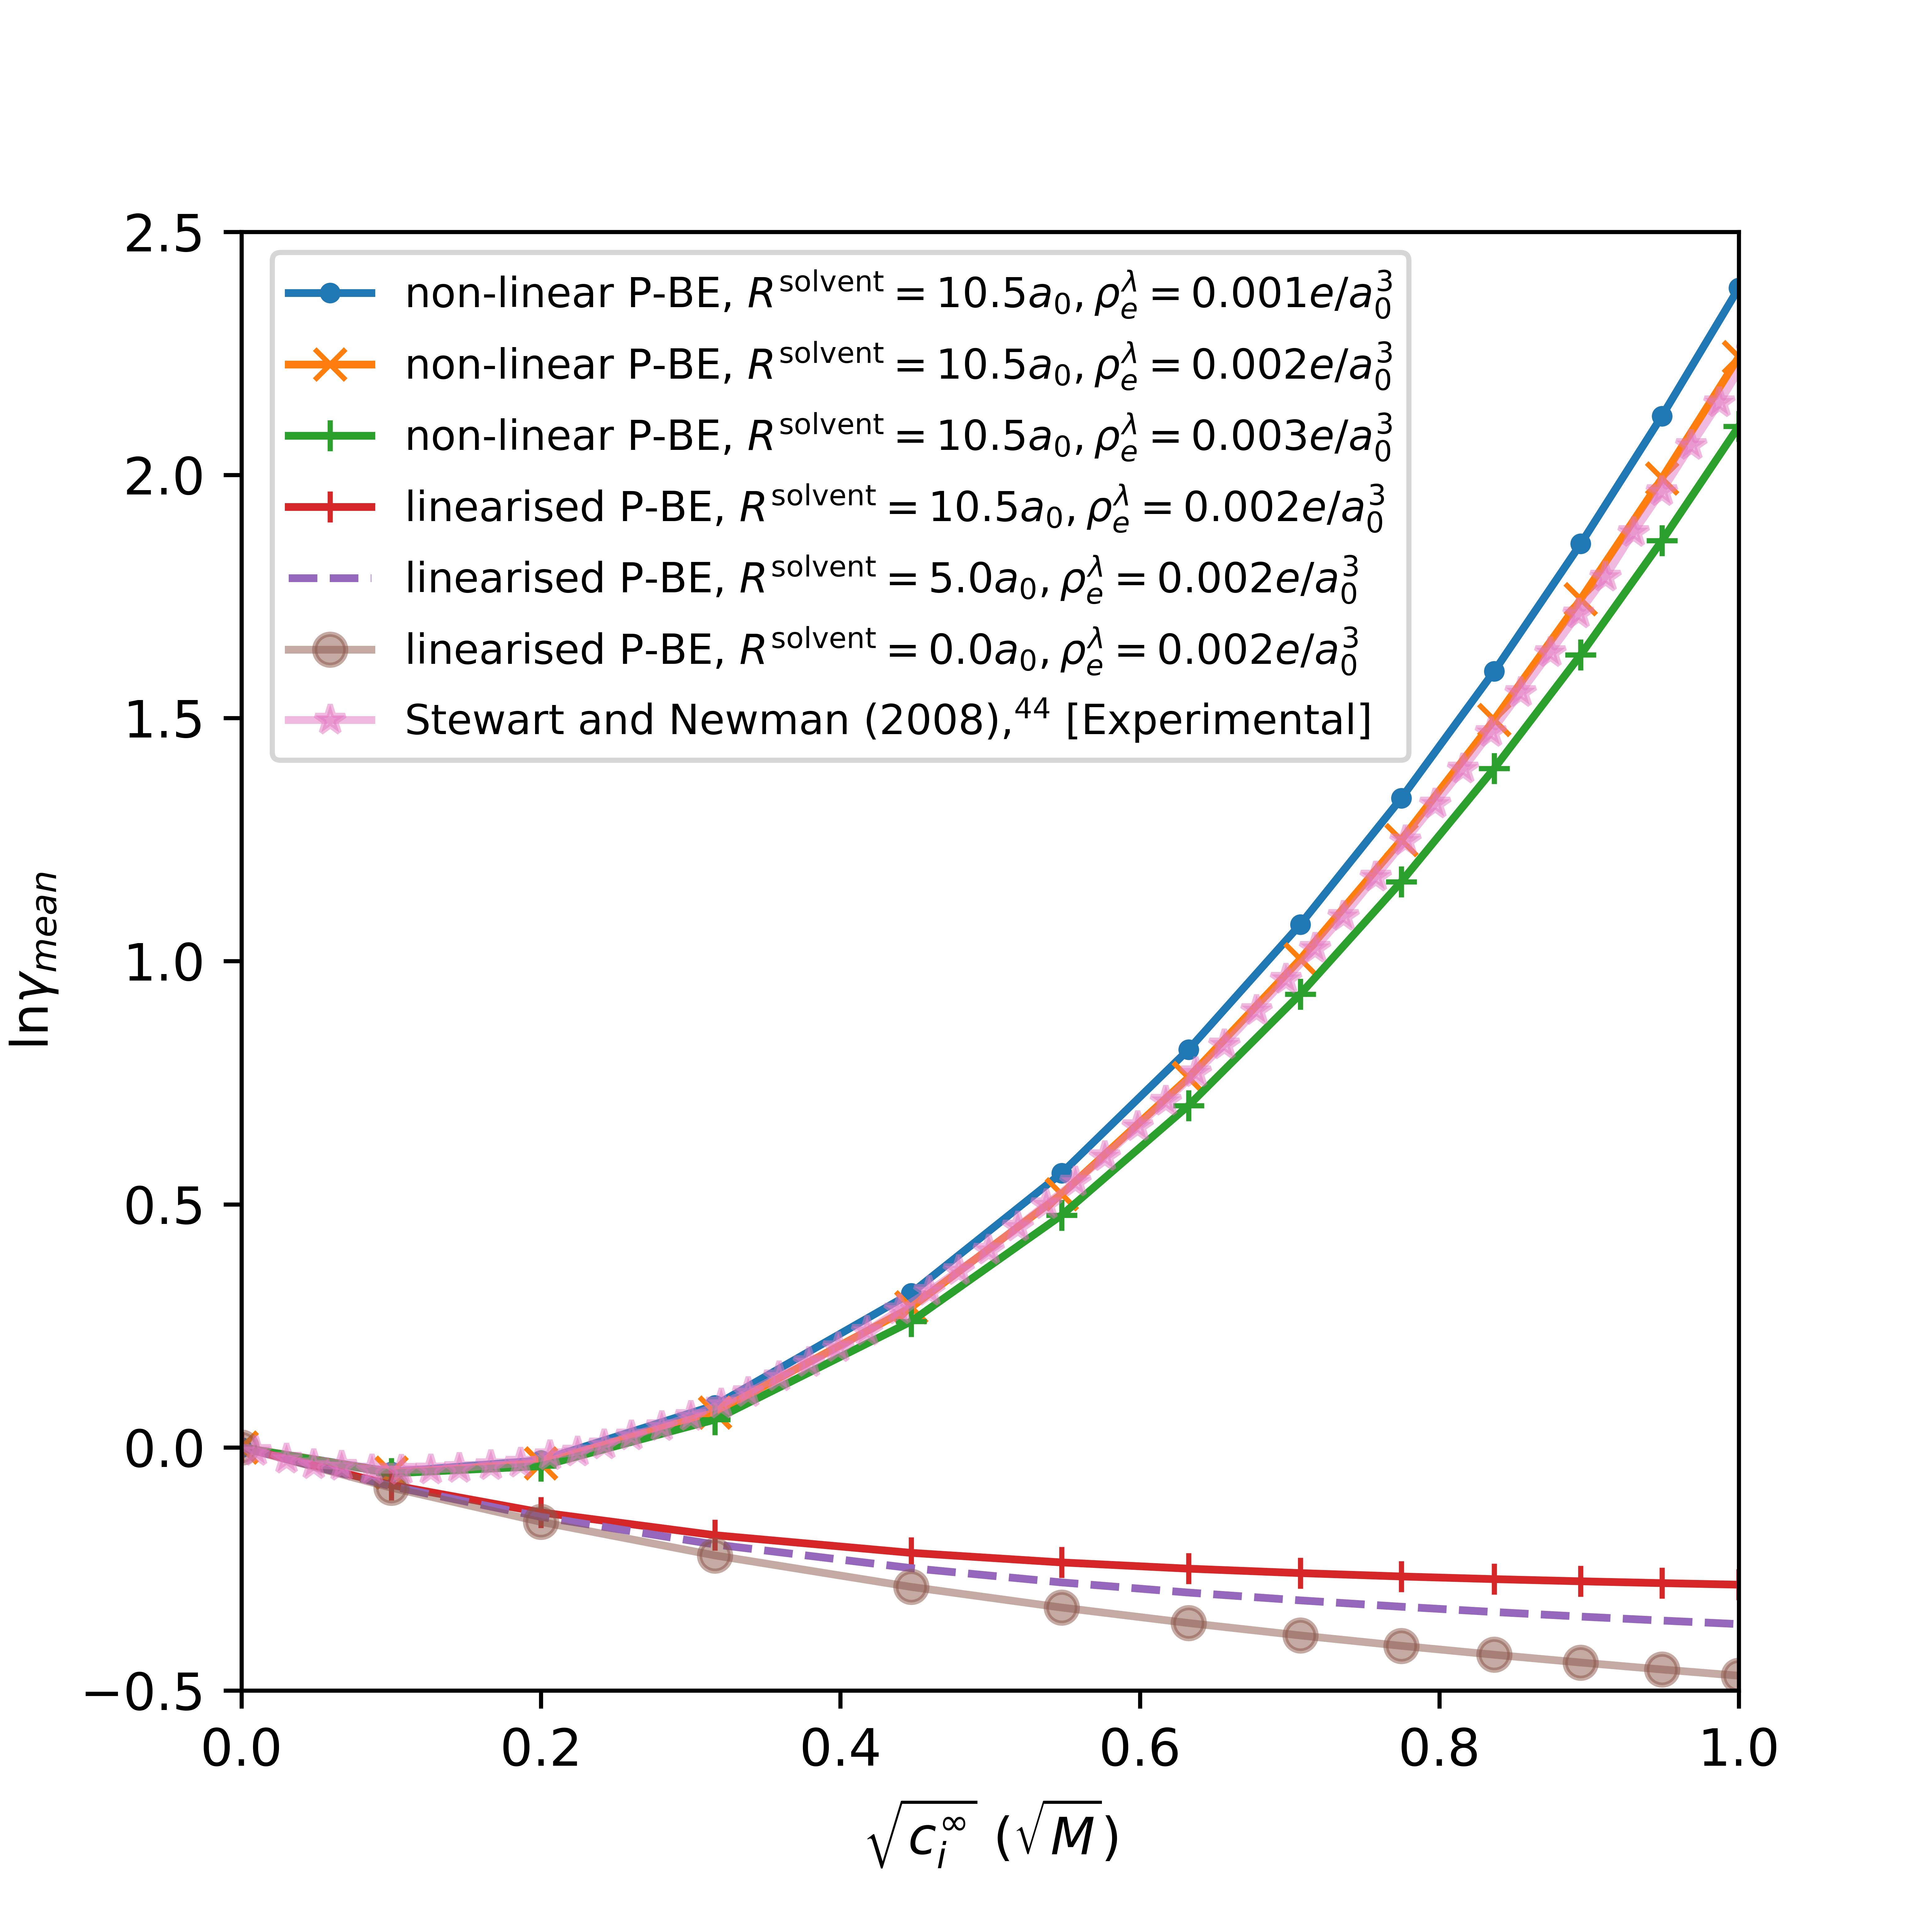
\includegraphics[scale=1]{figures/lipf6.png}
    \caption{Mean activity coefficients for LiPF$_6$ in ethylene carbonate at 308~K as a function of concentration and for different values of the atomic electronic density isovalue parameter which determines the extent of the accessibility function. Calculations with the linearized approximation to P-BE are also shown. Reproduced from Ref. \citenum{Dziedzic2020}}
    \label{fig:ac}
\end{figure}
    
\subsubsection{Outlook and challenges}
\begin{itemize}
    \item challenges - interatomic potentials for classical MD
    \item limitation of liquid electrolytes
\end{itemize}

\subsection{Solid Electrolytes}

\subsubsection{Introduction}
Lead: Arihant
Contributions: Rana, Lucy
% Different types of structures currently being worked on (argyrodites, garnets, perovskites, lisicons, nanocomposites), where each of these are in terms of conductivity and practical use, and what electrode materials they can be used with (if specific).
% cite review papers on solid electrolytes

Solid electrolytes have attracted considerable attention as an alternative to highly flammable liquid electrolytes, significantly improving device safety and with the potential to improve energy and power densities. \cite{janek_solid_2016, culver_designing_2018, famprikis_fundamentals_2019, goodenough_li-ion_2013} The high ion conductivities of liquid electrolytes has, thud far, been unreachable for solid electrolytes, however, research efforts over the last decade have presented a limited number of promising candidates with high ionic conductivities ($>$1 mS cm$^{-1}$) as a potential competitive to liquid electrolytes.\cite{kanno_synthesis_2000,murayama_synthesis_2002,murayama_material_2004,minafra_influence_2019,bron_li_2013,whiteley_empowering_2014,huang_superionic_2019,yamane_crystal_2007,homma_crystal_2011} \citeauthor{Kamaya2011} have plotted ionic conductivity of all known solid electrolytes, presented in Figure \ref{fig:solid-electrolyte}. \cite{Kamaya2011} 

.... In this section, we review computational studies of ion mobility in solid electrolytes, broadly belonging to three chemical groups: oxides, sulfides, and others.

% Possibly we can select some of the below to mention. I think the Van de Ven review covers them all, but we can focus on a few.
% Oxides - NASICONs, LISICONS, perovskites (LLTO), Li garnets
% sulfides - glass ceramics, thio-LISICON (LGPS), argyrodites.
% Others - nanocomposites?, nitrides, oxynitrides (LiPON), antiperovskites

\begin{figure}[h]
    \centering
    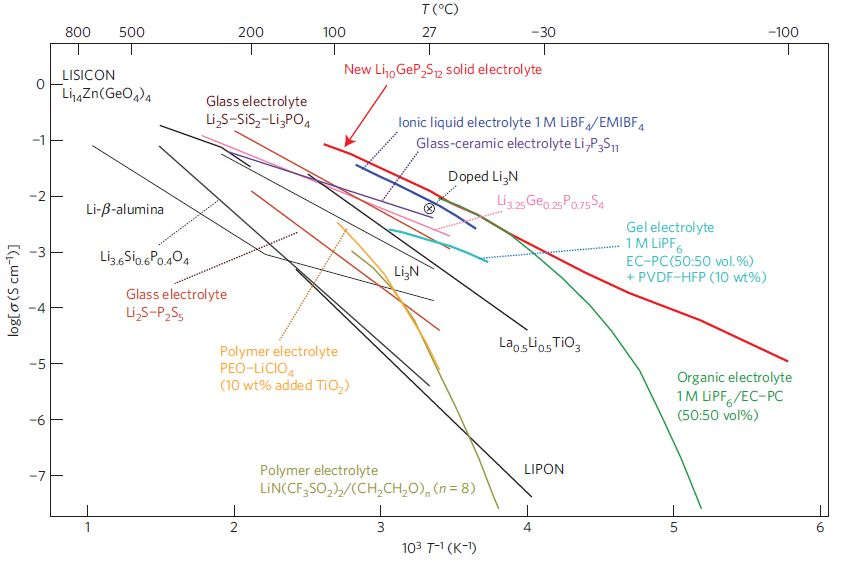
\includegraphics[scale=0.65]{figures/kamaya.jpg}
    \caption{Ionic conductivity of different solid electrolytes from Ref. \citenum{Kamaya2011}}
    \label{fig:solid-electrolyte}
\end{figure}
\clearpage

\subsubsection{Diffusion properties}

\subsubsubsection{Li-Argyrodites (Lucy)}

Lithium argyodites, (Li$_6$PS$_{5}X$, $X$= Cl, Br, or I), are among the promising candidates for solid electrolytes, reportedly reaching ionic conductivities of $10^{-2}$ to $10^{-3}$ Scm$^{-1}$, comparative to liquid electrolytes. \cite{deiseroth_li6ps5x_2008} They belong to a broader chemical group of sulfide based solid electrolytes, which also include glass ceramics \re{references and example} and thio-LISICONs such as LGPS \re{again references}.

\begin{itemize}
    \item anion disorder
    \item Li concentration - Li site occupation
    \item cation/anion doping
\end{itemize}
\newline
\newline

\subsubsubsection{LGPS (Arihant)}

diffusion in superionic conductors like LGPS,\cite{Bhandari2016} LLZO, etc. (Arihant)
%LLZO could be drop if needed
\begin{figure}
    \centering
    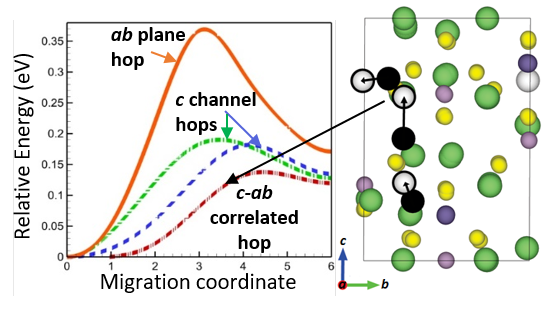
\includegraphics[scale=1.2]{figures/lgps.png}
    \caption{Energy barrier for Li-ion diffusion in LGPS solid electrolyte calculated using NEB method. Ref. \citenum{Bhandari2016}}
    \label{fig:my_label}
\end{figure}


\subsubsubsection{Nanocomposites (Rana)}

Due to attractive mechanical, electrical, optical, and magnetic properties nanocomposite oxide materials represent a new generation of advanced materials. They often show enhanced conductivity compared to the single-phase ceramic oxides which makes them suitable candidates as electrolytes for the future all solid state batteries. For example, Li$_2$O:B$_2$O$_3$ \cite{Heitjans_2003,Indris2000,Indris2002} and Li$_2$O:Al$_2$O$_3$ nanocomposites \cite{B300908D} have higher ionic conductivities than nanocrystalline Li$_2$O, although B$_2$O$_3$ and Al$_2$O$_3$ are insulators. The ionic conductivity shows a maximum at about 50 \% of B$_2$O$_3$/Al$_2$O$_3$ content. This surprising behaviour was attributed to the increased fraction of structurally disordered interfacial regions and the enhanced surface area of the nanosize particles \cite{Heitjans_2003}. The nanocomposites contain three types of interfaces (Fig.\ref{fig:LBO} (a)), i.e., interfaces between the ionic conductor grains (green lines), between the insulator grains (black lines) and between the ionic conductor and the insulator grains (red lines). The latter can lead to surprising effects in the conductivity of composite materials. In this case, the highly conducting interface region can act as a bridge between two Li$_$O grains not in direct contact with each other, opening up additional paths for Li ions. The conductivity enhancement in the interfacial regions may have different origins, e.g. the formation of space charge layers, an enhanced concentration of dislocations, or defects or the formation of new phases.

\begin{figure}
    \centering
    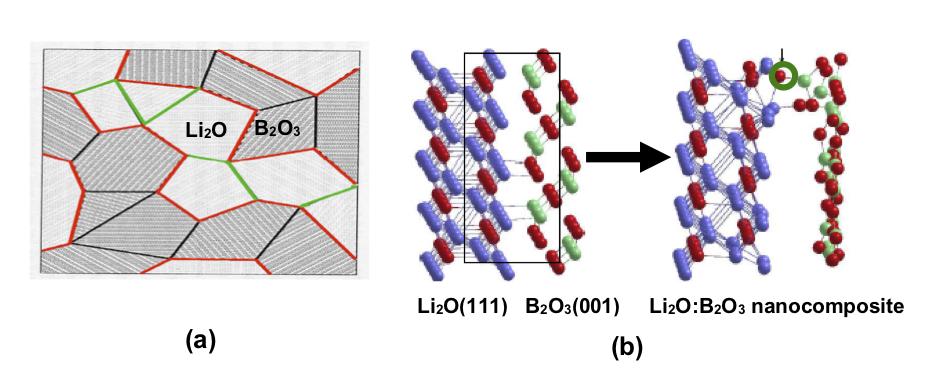
\includegraphics[scale=1]{figures/Islam-Fig-Li2O-B2O3.png}
    \caption{(a) Schematic diagram of Li$_2$O and B$_2$O$_3$ interface (Reproduced from ref. \citenum{Heitjans_2003}). (b) Atomistic model of Li$_2$O:B$_2$O$_3$ nanocomposite ref. \citenum{Rana-JPCM-2012}.}
    \label{fig:LBO}
\end{figure}

Here we review a previous theoretical study on the stability and enhanced ionic conductivity at Li$_2$O:B$_2$O$_3$ nanocomposites \cite{Rana-PRL-2007,Rana-JPCM-2012}. The interface of Li$_2$O:B$_2$O$_3$ nanocomposite was modeled by the combination of two favorable surfaces of Li$_2$O and B$_2$O$_3$. After full structural optimization, it was observed that Li--O bonds are weakened and simultaneously B--O bonds are formed at the boundary between the two surfaces (Fig. \ref{fig:LBO} (b)). An oxygen atom from the Li$_2$O surface (on the right, marked by a green circle) is pulled from the surface layer towards a neighboring boron atom of the B$_2$O$_3$ surface. This preference of oxygen bonding with B (or Al in Li$_2$O:Al$_2$O$_3$) plays a key role in generating low-coordinated Li. As a consequence of this dislocation, the coordination of a Li atom in the second layer is reduced from four to three. 

The defect properties were investigated in the interface region. It was observed that the removal of surface oxygen from Li$_2$O is responsible for the increased vacancy defect concentration in Li$_2$O:B$_2$O$_3$ (or Li$_2$O:Al$_2$O$_3$) nanocomposite materials. Therefore the nanocomposites of ionic compounds (containing weakly bound and therefore mobile cations) with highly covalent compounds (with strong metal- or nonmetal-oxygen bonds) are in general promising candidates for high ionic conductivity. The model calculations showed that the most likely mechanism for Li$^+$ migration was in a zigzag pathway rather than in a straight line along a direction parallel to the interface plane. The average calculated activation energy for Li$^+$ migration in the Li$_2$O:B$_2$O$_3$ interface is similar to the experimental values of bulk Li$_2$O, Li$_2$O:B$_2$O$_3$ and Li$_2$O:Al$_2$O$_3$ nanocomposites. Therefore the experimentally observed enhanced Li mobility in the Li$_2$O:B$_2$O$_3$ interface region is thermodynamically and not kinetically controlled.


\subsubsection{Interface stability (Arihant)}
%Solid-solid interfaces. Possibly keep as a section or merge with the outlook below.

\subsubsection{Outlook and challenges}



\section{Cathodes (Lucy/Rana/Hui)}
material: LiFePO4
\subsection{Introduction and historical context}
Lead: ?

\subsection{Bulk Properties}
\subsubsection{Bulk structural properties}
Lead: ?
\begin{itemize}
    \item cation ordering in layered structures (Rana)
    \item order/disorder
    \item dopants?
    \item different structures (layered/spinel/rock-salt)
    \item calculating shear/bulk/Young's modulus (DFT/classical)
    \item stress-strain properties (Lucy/Sayle)
\end{itemize}

\subsubsection{Bulk diffusion properties}
Lead: Lucy
\newline
Materials: LiNiO2 (Lucy+Rana), LiMnO2(Sayle), other materials not covered by the NMC review i.e. review other's work

\begin{itemize}
    \item From DFT to Classical MD and possibly Monte Carlo examples.
    \item DFT - hopping frequencies, diffusion mechanisms
    \item DFT+Classical diffusion coefficients
    \item Classical (+Monte Carlo?) diffusion at grain boundaries.
    \item temperature effects
\end{itemize}

\subsubsection{Thermal, electronic, and vibrational properties of cathodes}
Lead: Hui

\subsection{Surfaces and Interfaces (Arihant)}
Although, the cathode-electrolyte interface (CEI) is quite thinner than the SEI at the anode, it is still quite complex in structure and composition.\cite{Gauthier2015, Edstrom2004} DFT based simulations can provide insight into adsorption trends,\cite{Bhandari2020} reaction pathways and energetics,\cite{Tebbe2015a, Tebbe2015b} migration barrier for Li-ion transfer,\cite{Bhandari2019} etc. The electrolyte in the Li-ion battery, is typically a Li salt such as LiPF$_6$ in an organic carbonate solvent, such as ethylene carbonate (EC), propylene carbonate (PC), diethyl carbonate (DEC) or dimethyl carbonate (DMC). The LiPF$_6$ electrolyte reacts with trace amounts of moisture to form HF,\cite{Tebbe2015a} which is highly corrosive and reacts with the cathode surface to form fluoride-based products.\cite{Tebbe2015b} The organic carbonate solvent  also react with the cathode surface to form a series of decomposition products.\cite{Tebbe2016} The adsorption of organic carbonate and fluoride-based products is the first step in the series of reactions that lead to the formation of CEI. The decomposition reaction of cyclic organic carbonates proceeds via ring opening. The energy barrier for the ring opening reaction has been predicted to be around 0.62 eV on (100) LiMn$_2$O$_4$ surfaces,\cite{Leung2012} over 1 eV on (101$\Bar{4}$) LiCoO$_2$ surfaces.\cite{Tebbe2016} and around 0.29 eV on (101$\Bar{4}$) Li(Ni,Mn,Co)O$_2$ surfaces,\cite{Xu2017} via the NEB method.\cite{JONSSON1998} While experimental studies on composition of CEI has shown presence of both solvent-decomposition and fluoride-based products on most oxide cathodes, such as LiMn$_2$O$_4$, LiNiO$_2$ LiCoO$_2$ and LiNi$_0.8$Co$_0.2$O$_2$, no solvent reaction or solvent decomposition products are detected on LiFePO$_4$.\cite{Edstrom2004, Malmgren2010} Recent calculations of adsorption energies based on DFT have shown that adsorption preference of HF over EC leads to the entire LiFePO$_4$ nano-particle being covered by fluoride based products, which further their leads to dominant in the CEI.\cite{Bhandari2020} Based on DFT simulations, it is also possible to design suitable coatings in order to prevent cathode degradation,\cite{Tebbe2015b} These calculations can shortlist effective candidate materials for experiments and guide experiments. Thus the atomistic methods not only provide the necessary insights needed in order to rationalize the experimental observations but novel solutions to mitigate cathode degradation.

Apart from the complexity of structure of the CEI, another challenge is to understand the Li ion migration mechanism at the CEI. The rate capability of Li-ion batteries is crucially influenced by Li-ion diffusion within bulk electrodes and electrolyte, and Li-ion transfer across the electrode-electrolyte interfaces. Relative magnitudes of both bulk and interfacial diffusion energy barriers are essential in order to identify the rate-limiting component in overall Li-ion transport process. The Li-ion conductivity in the bulk of electrodes and electrolytes has been well studied in literature and it is well known that Li-ionic conductivity in electrolytes (1 S/cm) is several orders of magnitude higher than that in the electrode materials (10$^{-7}$-10$^{-2}$ S/cm).\cite{Park2010, VanDerVen2013} However, the kinetics at the electrode-electrolyte interface is less understood due to the complex structure of the interface and the unknown mechanism of Li-ion transfer from the bulk electrolyte into the bulk electrode. Recent DFT-NEB calculations have estimated an energy barrier of 756 meV for Li to move from a near-surface solvated cluster to a sub-surface vacancy in the LiFePO$_4$ cathode material.\cite{Bhandari2019} Due to preferential adsorption of fluoride on LiFePO$_4$ surfaces,\cite{Edstrom2004, Bhandari2020} the energy barrier has been found to decrease to 410 meV in presence of fluoride. Nevertheless, the interfacial energy barrier is quite higher than that in the bulk cathode material, which is estimated to be around 270-290 meV.\cite{Morgan2004,Dathar2011} This shows, a rate-limiting behaviour of the interface in the overall Li-ion diffusion process in the Li-ion batteries. The study motivates further such investigation on other cathode materials, and with the recently developed advanced-methods for characterizing the interface as described in sec. \ref{sec:dft+cont}.   

\section{Outlook}
\begin{itemize}
    \item Linking atomistic modelling to continuum models and/or experiment
    \item Challenging areas - interfaces, heterogeneity (grain boundaries, defects), modelling charging and discharging (materials in working conditions), 
    \item Further developments in atomistic methods of batteries
\end{itemize}


\section*{ORCID ids}
% Please place ORCID ids here.
Lucy M. Morgan : https://orcid.org/0000-0002-6432-3760 \newline
Michael P. Mercer: https://orcid.org/0000-0001-7578-3554 \newline
Chao Peng: https://orcid.org/0000-0003-3099-2808 \newline
Chris-Kriton Skylaris: https://orcid.org/0000-0003-0258-3433 \newline
Hui Yang: https://orcid.org/0000-0002-7890-5411 \newline
Mazharul M Islam: https://orcid.org/0000-0002-5638-8265 \newline
Arihant Bhandari: https://orcid.org/0000-0002-2914-9402 \newline


%%%%%%%%%%%%%%%%%%%%%%%%%%%%%%%%%%%%%%%%%%%%%%%%%%%%%%%%%%%%%%%%%%%%%
%% The "Acknowledgement" section can be given in all manuscript
%% classes.  This should be given within the "acknowledgement"
%% environment, which will make the correct section or running title.
%%%%%%%%%%%%%%%%%%%%%%%%%%%%%%%%%%%%%%%%%%%%%%%%%%%%%%%%%%%%%%%%%%%%%
\begin{acknowledgement}

Please use ``The authors thank \ldots'' rather than ``The
authors would like to thank \ldots''.


\end{acknowledgement}

%%%%%%%%%%%%%%%%%%%%%%%%%%%%%%%%%%%%%%%%%%%%%%%%%%%%%%%%%%%%%%%%%%%%%
%% The same is true for Supporting Information, which should use the
%% suppinfo environment.
%%%%%%%%%%%%%%%%%%%%%%%%%%%%%%%%%%%%%%%%%%%%%%%%%%%%%%%%%%%%%%%%%%%%%
\begin{suppinfo}

This will usually read something like: ``Experimental procedures and
characterization data for all new compounds.

\end{suppinfo}

%%%%%%%%%%%%%%%%%%%%%%%%%%%%%%%%%%%%%%%%%%%%%%%%%%%%%%%%%%%%%%%%%%%%%
%% The appropriate \bibliography command should be placed here.
%% Notice that the class file automatically sets \bibliographystyle
%% and also names the section correctly.
%%%%%%%%%%%%%%%%%%%%%%%%%%%%%%%%%%%%%%%%%%%%%%%%%%%%%%%%%%%%%%%%%%%%%
\bibliography{biblio}

\end{document}